\setcounter{chapter}{2}
\chapter{Experiments}

    The following chapter will explain the methodology and the results of the various experiments undertaken to develop, validate, and characterize the V2 thruster. Argon gas was used as the propellant in all cases, due to its low cost, safety, and ease of ionization.

    \section{Static LSP validation}

        \subsection{V1 LSP spark initiation}

            For spark initiation to work reliably, the laser focus and the spark must both be aligned in space and in time. To resolve the spark spatially, the Photron SA5 camera was placed in front of the V1 test section instead of the laser, looking axially into the test section. This would be the point of view of the laser collimator during a Laser-Supported Plasma (LSP) shot. \autoref{fig:spark composite} shows a composite photo of the added opacities of five spark discharges (without laser). Each frame of the video has an opacity of $1/N$, with $N$ being the total number of frames to add. This gave an average position of the spark, which is slightly to the left of the electrodes' centerline.

            \begin{figure}[!ht]
                \centering
                \begin{subfigure}[t]{0.25\textwidth}
                    \centering
                    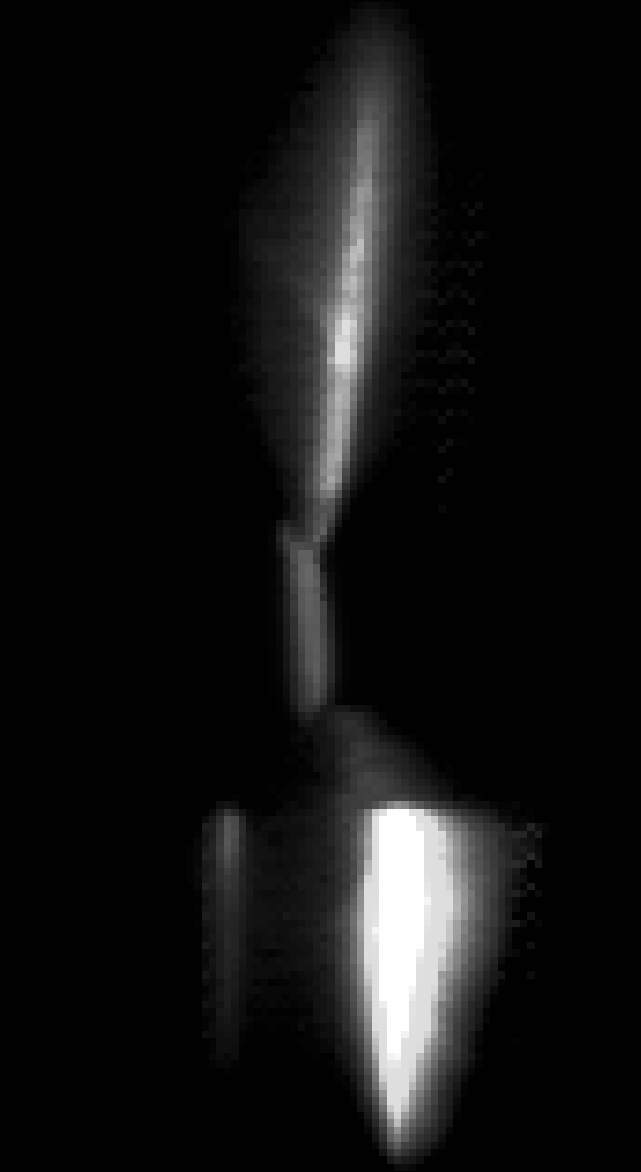
\includegraphics[width=\textwidth]{assets/4 experiments/Composite photo spark.png}
                    \caption{Composite photo showing spark between two electrodes. The spark gap is approximately \qty{0.8}{mm}.}
                    \label{fig:spark composite}
                \end{subfigure}
                \hfill
                \begin{subfigure}[t]{0.45\textwidth}
                    \centering
                    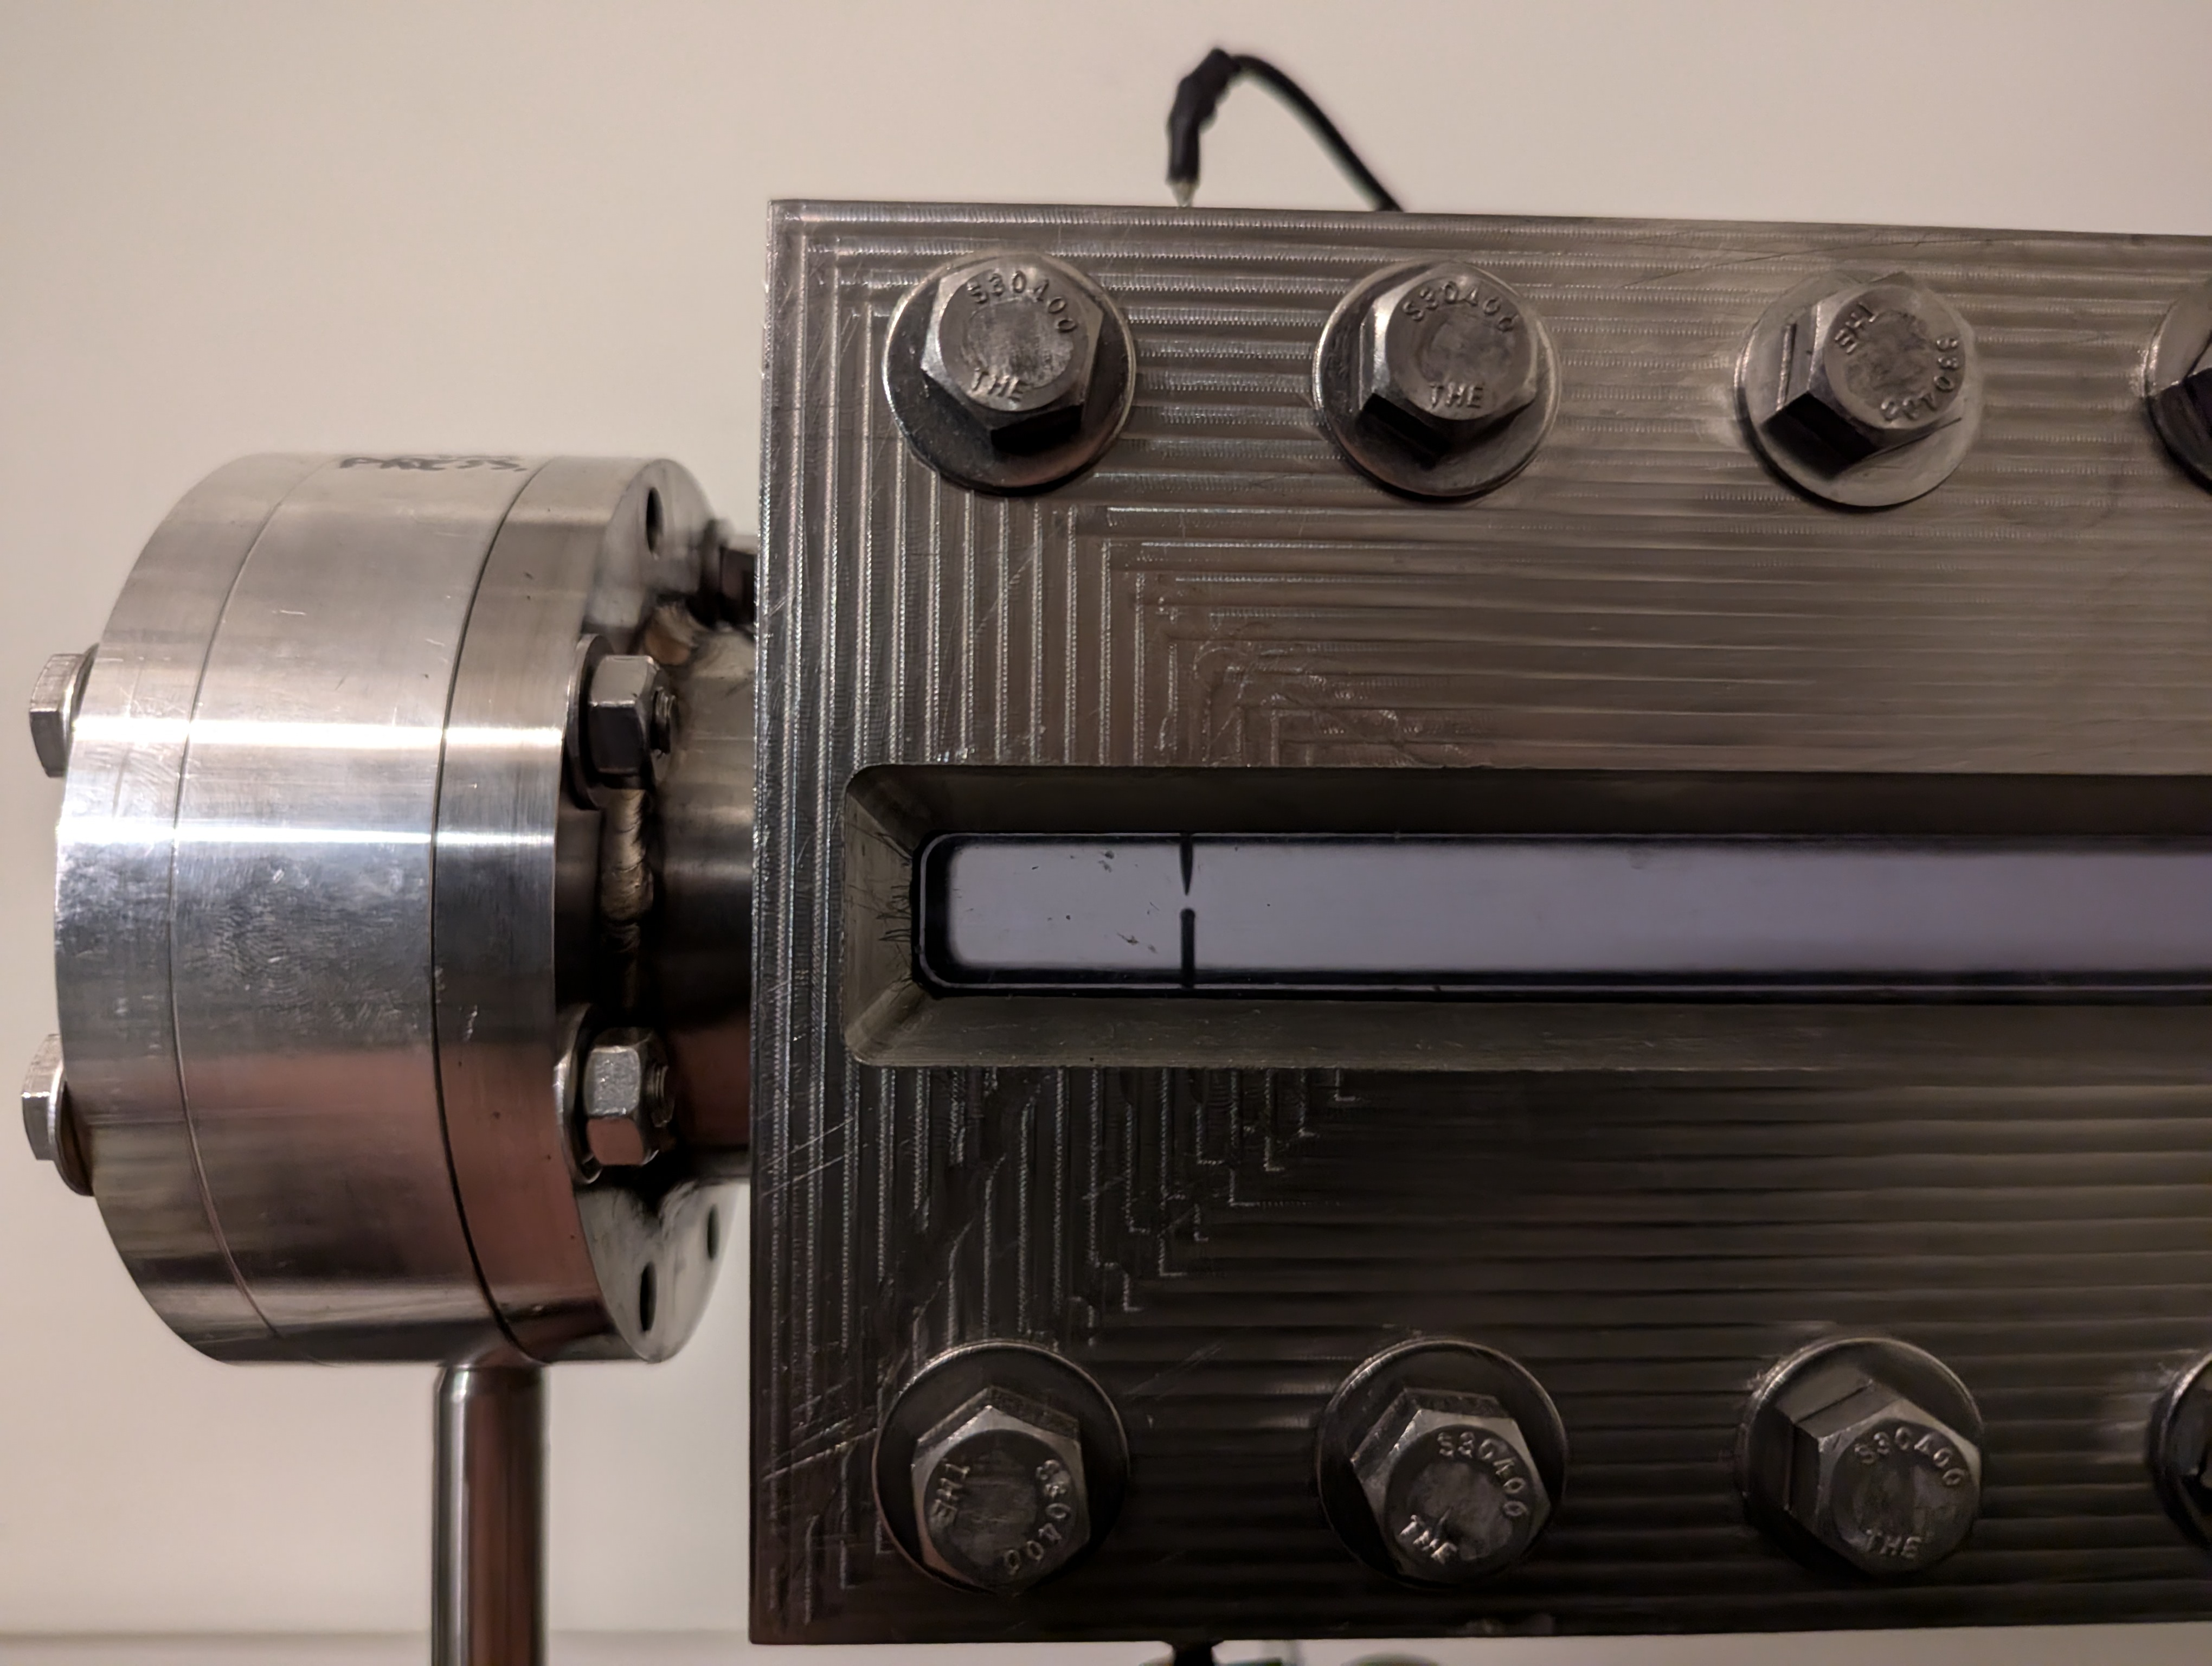
\includegraphics[width=\textwidth]{assets/4 experiments/V1 opposing electrodes.jpg}
                    \caption{Front of V1 test section showing electrode position. This view is rotated 90\degree from \autoref{fig:spark composite}}
                    \label{fig: standard view of electrodes}
                \end{subfigure}
                \caption{V1 spark alignment}
            \end{figure}
            
            Using the thickness of the electrode (\qty{1.55}{mm}) as a reference, the spark gap's length is \qty{0.8}{mm} and the average spark is \qty{0.2}{mm} wide. Timing data was also recorded for the spark by the high-speed camera. To align the laser focus to the spark in time, the laser was reinstalled, and the camera was placed back to its normal position looking into the side of the test section (seen in \autoref{fig: standard view of electrodes}). The beam was then focused on one of the electrodes at low power. This caused the electrode to glow white-hot when the laser was on. The timings presented in \autoref{fig: Signal timing diagram} were determined by this investigation.

            \begin{figure}[!ht]
                \centering
                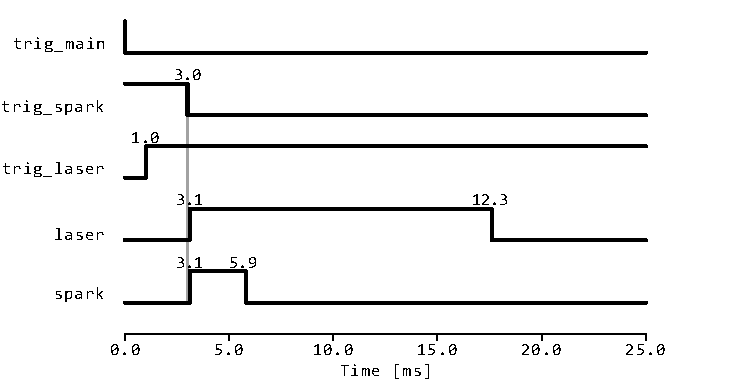
\includegraphics[width=0.75\textwidth]{assets/4 experiments/timings.pdf}
                \caption{Signal timing diagram. The \textit{trig} prefix denotes triggering signals. The component is active when the line is high. Timings in \unit{ms} are also indicated on the figure.}
                \label{fig: Signal timing diagram}
            \end{figure}

            With the position of the laser aligned to the spark and the timings synchronized, QCW LSP spark initiation in V1 was achieved with a \qty{200}{mm} focal length lens at 100\% power (\qty{3079}{W}) and a pressure of \qty{20}{bar}, as seen in \autoref{fig:V1_spark_initiation_frames}.
            
            \begin{figure}[h]
    \centering
    \begin{subfigure}[t]{0.3\textwidth}
        \centering
        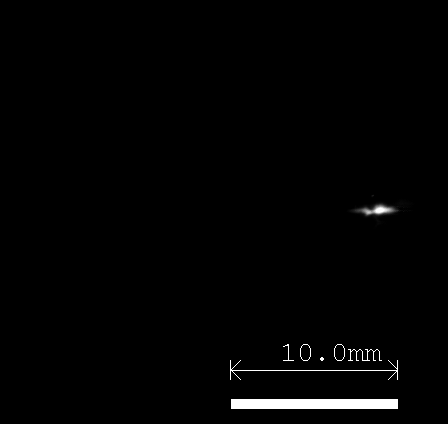
\includegraphics[width=\textwidth]{assets/4 experiments/V1 Spark Ignition Frames/LSP142_SPRK15_Fr32.bmp}
        \caption{\qty{3.2}{ms}}
        %\label{fig:V1_ignition_frames_16}
    \end{subfigure}
    \hfill
    \begin{subfigure}[t]{0.3\textwidth}
        \centering
        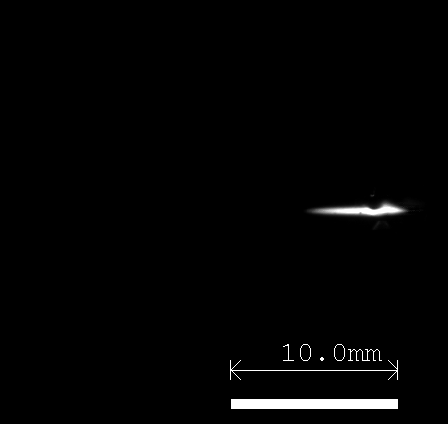
\includegraphics[width=\textwidth]{assets/4 experiments/V1 Spark Ignition Frames/LSP142_SPRK15_Fr33.bmp}
        \caption{\qty{3.3}{ms}}
        %\label{fig:ignition_frames_17}
    \end{subfigure}
    \hfill
    \begin{subfigure}[t]{0.3\textwidth}
        \centering
        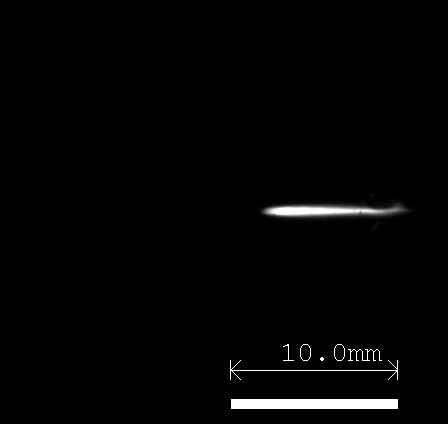
\includegraphics[width=\textwidth]{assets/4 experiments/V1 Spark Ignition Frames/LSP142_SPRK15_Fr35.bmp}
        \caption{\qty{3.5}{ms}}
        %\label{fig:ignition_frames_18}
    \end{subfigure}
    \begin{subfigure}[t]{0.3\textwidth}
        \centering
        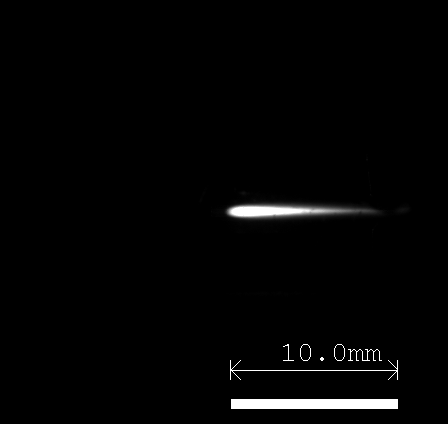
\includegraphics[width=\textwidth]{assets/4 experiments/V1 Spark Ignition Frames/LSP142_SPRK15_Fr38.bmp}
        \caption{\qty{3.8}{ms}}
        %\label{fig:ignition_frames_19}
    \end{subfigure}
    \hfill
    \begin{subfigure}[t]{0.3\textwidth}
        \centering
        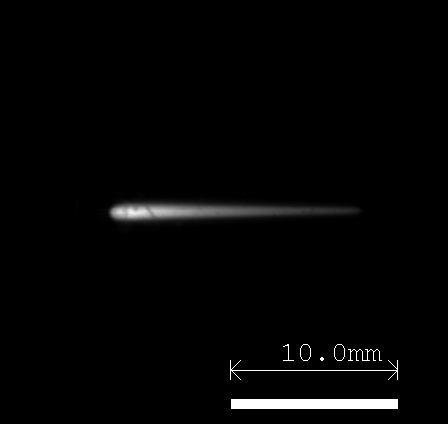
\includegraphics[width=\textwidth]{assets/4 experiments/V1 Spark Ignition Frames/LSP142_SPRK15_Fr69.bmp}
        \caption{\qty{6.9}{ms}}
        %\label{fig:ignition_frames_20}
    \end{subfigure}
    \hfill
    \begin{subfigure}[t]{0.3\textwidth}
        \centering
        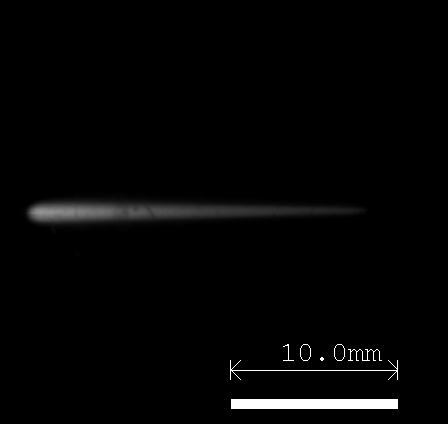
\includegraphics[width=\textwidth]{assets/4 experiments/V1 Spark Ignition Frames/LSP142_SPRK15_Fr130.bmp}
        \caption{\qty{13.0}{ms}}
        %\label{fig:ignition_frames_21}
    \end{subfigure}
    \caption{LSP spark initiation: \qty{3080}{W}, \qty{20}{bar}. \shotsettings{LSP142\_SPRK15}{0.1?? CHANGE}{22}{2048}}
    \label{fig:V1_spark_initiation_frames}
\end{figure}
            
            The LSP is initiated at \qty{3.2}{ms}, as soon as the spark is discharged. The front of the LSP moves towards the left (upstream, towards the laser), until the end of the QCW laser pulse at \qty{13}{ms}. Once the laser ends its emission, the LSP dies down within two frames (\qty{0.2}{ms}).
            % I could include here the dynamic pressure rise of the LSP.

        \subsection{\ce{NO2} seeding}

            \todo{Add context to this section}
            % If you want to present the NO2 work, you'll need to: Explain attenuation/absorption coefficient as it appears in Beer-Lambert law and how this defines the length scale over which absorption occurs. Explain how absorption coefficient is derived from the cross-section of the molecule, which will involve using the HITRAN database, etc. It is not acceptable to just say "we added NO2" and reference it off to some paper.}
            
            As the plasma emits in the ultraviolet (UV) range, it is necessary to seed with a gas that absorbs UV but not the infrared (IR) laser. \textcite{khanGasDetectionUsing2019} shows that \ce{NO2} and \ce{SO2} are two candidates. \ce{NO2} was first used as it was easy to produce in-house in significant quantities. The V1 system was set up with a vacuum pump connected to an outside air exhaust to safely vent the \ce{NO2} gas. The pump was also used to bring the pressure in the test section down to a rough vacuum before introducing the gasses.

            %[Add absorption spectrum of NO2 from Gas Detection Using Portable Deep-UV Absorption Spectrophotometry: A Review or other place]

            Three control QCW LSP shots were done in pure argon and their dynamic pressure trace from the PCB transducer was recorded. Next, 0.55 bar of \ce{NO2}, or 200 mL at STP, was introduced into the chamber. V1 was then pressurized with argon to 20 bar. With the spark active, three LSPs were generated in the seeded atmosphere. The dynamic pressure rise of the seeded argon was approximately double the one seen in pure argon. The next two LSP shots were conducted with 0.24 bar (\qty{85}{ml} at STP) of \ce{NO2} and filled to 20.2 bar with argon. Again, higher pressure increases were observed, but slightly less than the \qty{0.55}{bar} shots. The chamber was finally half evacuated to 10.17 bar and then filled back to \qty{20.15}{bar} with argon. This would have brought the partial pressure of \ce{NO2} to \qty{0.12}{bar}. Two LSPs were initiated, with a higher pressure increase than pure argon, but less than the higher concentration \ce{NO2} shots. \autoref{fig:NO2_shots_analysis} presents the averages of these recorded pressure traces.

            \begin{figure}[!ht]
                \centering
                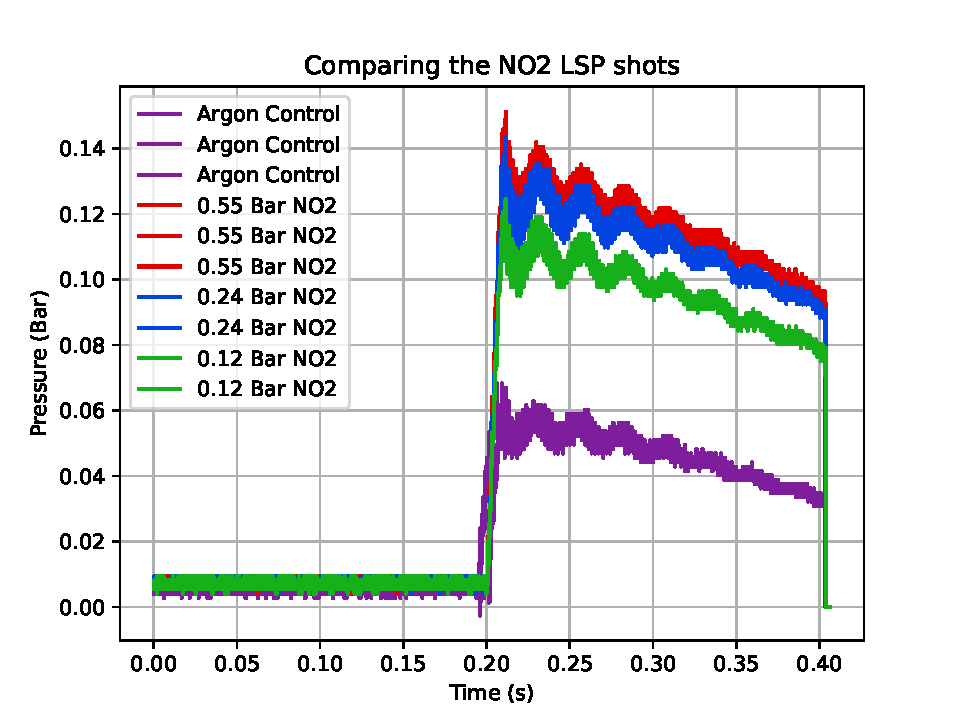
\includegraphics[width=0.75\textwidth]{assets/4 experiments/NO2_shots_analysis.pdf}
                \caption{Average dynamic pressure rise of QCW LSP shots in a mixture of \ce{NO2} and argon compared to that of pure argon QCW LSP. Initial pressure was \qty{20.15}{bar}. Values given in the legend are the partial pressure of \ce{NO2} seeding in the gas.}
                \label{fig:NO2_shots_analysis}
            \end{figure}

        \subsection{V2 LSP spark initiation and QCW LSP}

            For V2, the timings of the spark and laser pulse were kept the same as \autoref{fig: Signal timing diagram}. To align the laser focus spatially, the power meter was used as a screen to project the visible (red) alignment laser. By moving the V2 test section back and forth on the thrust stand rail, the field of view (FOV) of the shadows projected on the power meter can be modified, as seen in \autoref{fig:FOV}. The laser focus can then be moved with the translation stages, so the brightest spot matches the center of the electrodes' shadow.
            
            \begin{figure}[!ht]
                \centering
                \begin{subfigure}[t]{0.45\textwidth}
                    \centering
                    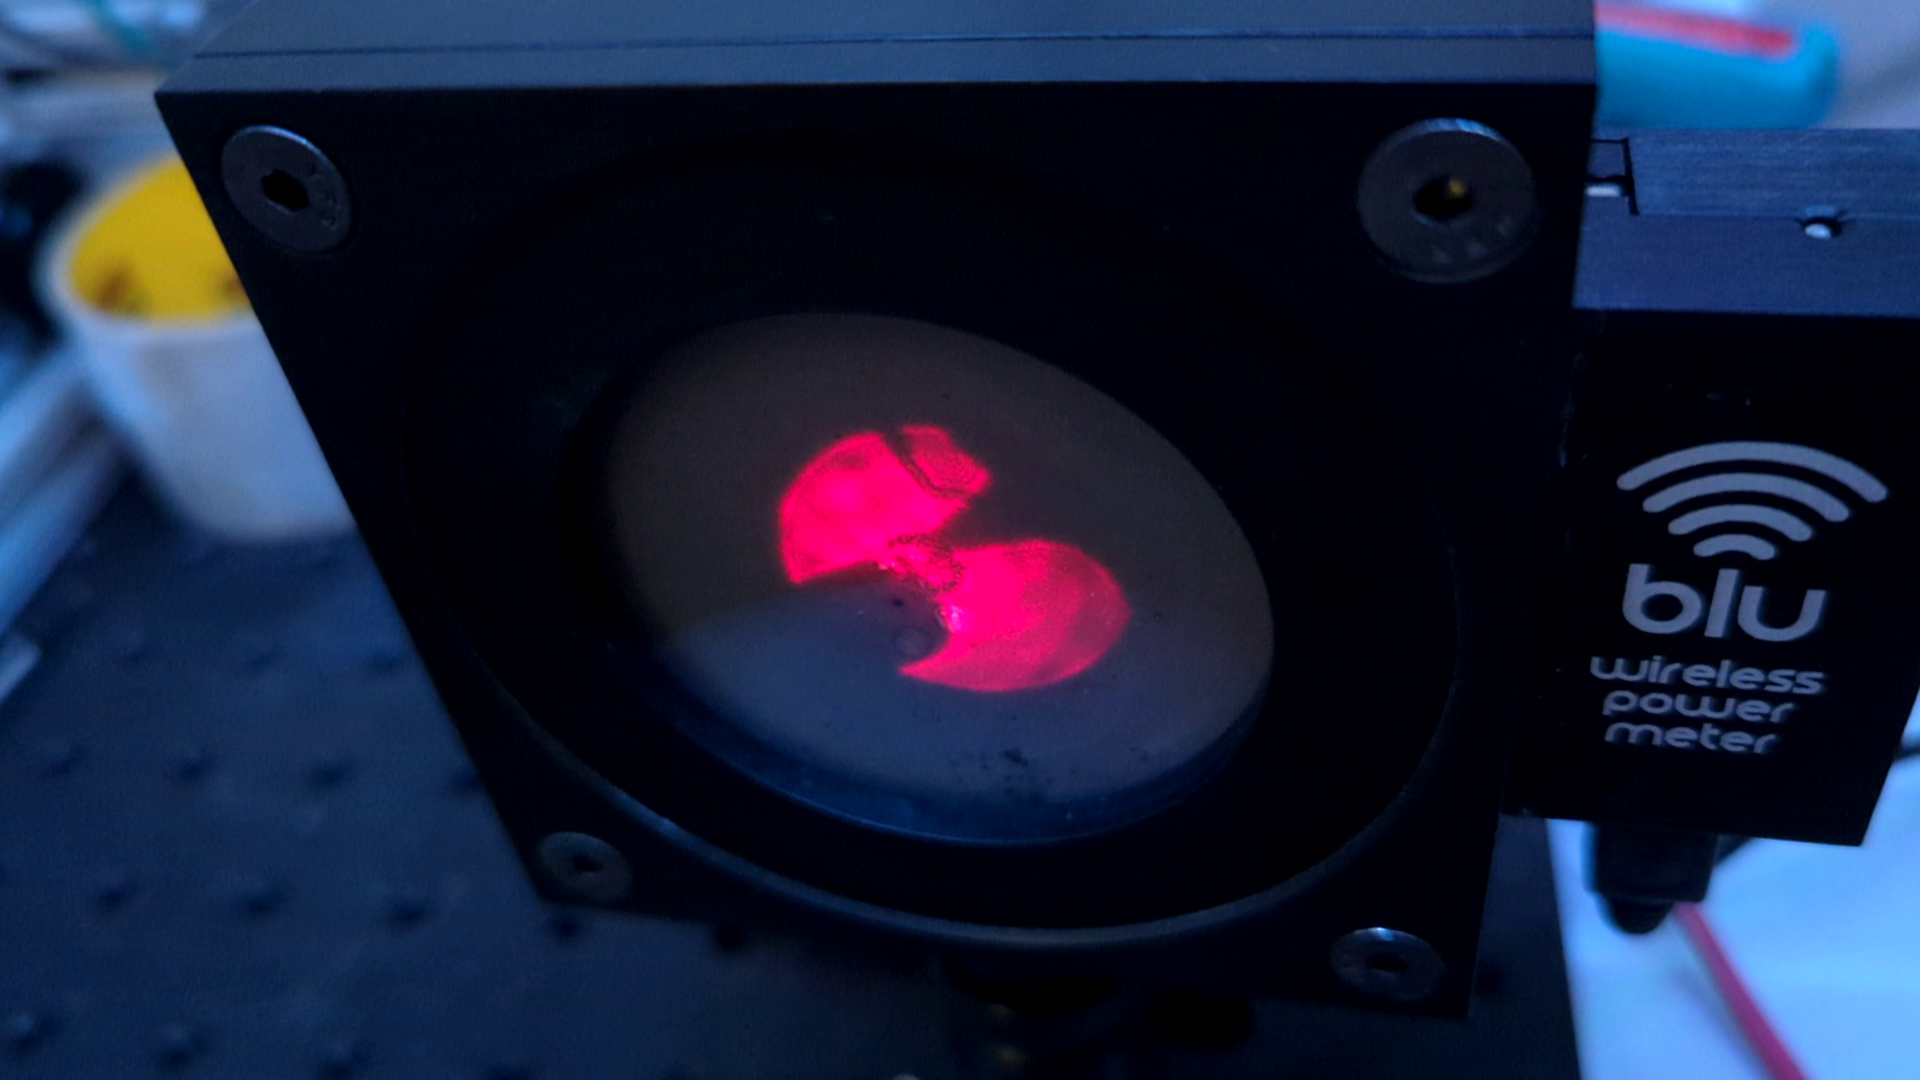
\includegraphics[width=\textwidth]{assets/4 experiments/V2 alignment 1.png}
                    \caption{V2 alignment, zoomed out}
                \end{subfigure}
                \hfill
                \begin{subfigure}[t]{0.45\textwidth}
                    \centering
                    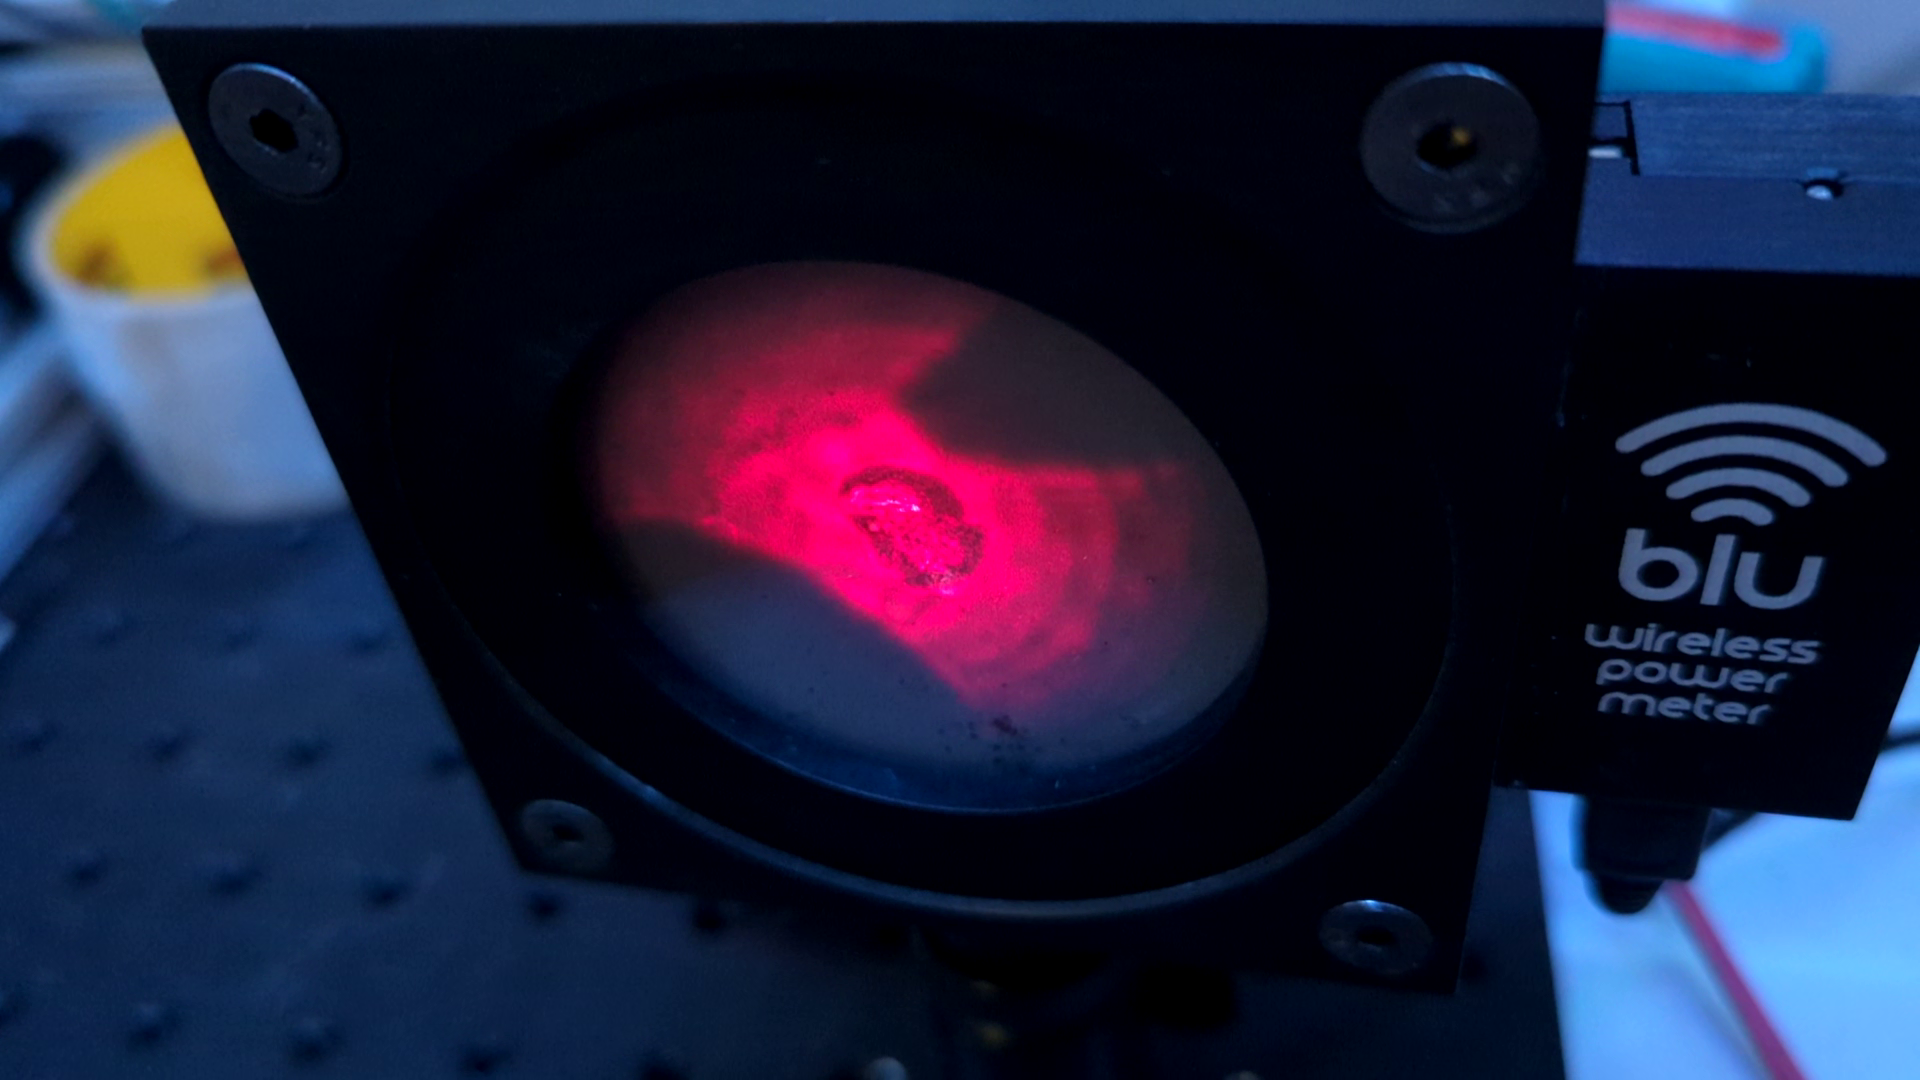
\includegraphics[width=\textwidth]{assets/4 experiments/V2 alignment 2.png}
                    \caption{V2 alignment, zoomed in}
                \end{subfigure}
                \caption{2 FOVs of alignment laser light on power meter. The aberration at the center of the red light is due to laser damage to the window.}
                \label{fig:FOV}
            \end{figure}

            Once the laser focus was aligned, QCW LSP initiation was confirmed in V2 by the Photron SA5 looking into the front of the thruster at an angle, and the PCB transducer recording the pressure rise. \autoref{fig: big flash}, taken by the webcam, shows the brightness of a full power QCW LSP. Note the bright plasma emission to the left of the image on the laser safety curtain.

            \begin{figure}[!ht]
                \centering
                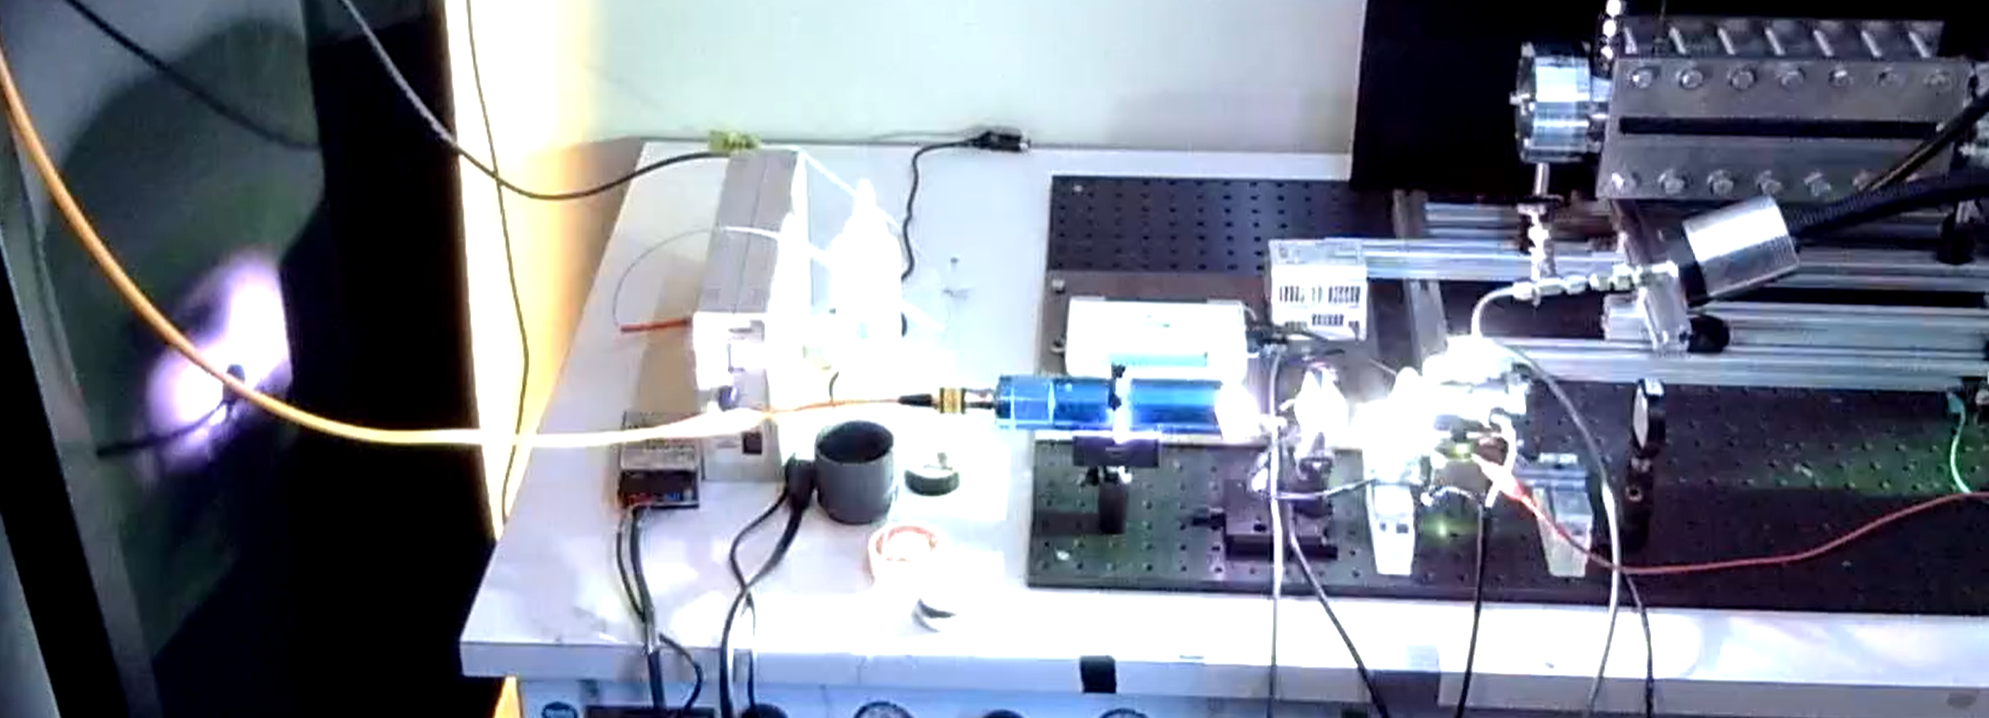
\includegraphics[width=\textwidth]{assets/4 experiments/holy jesus look at this.png}
                \caption{100\% power (\qty{3079}{W}) QCW LSP shot}
                \label{fig: big flash}
            \end{figure}

        \subsection{Optical experiments: going from QCW to CW LSP}

            Due to the low continuous laser power in this experiment compared to others in the literature, increasing the laser flux with a small focus is critical. The real amount of power in the pulsed shots was measured to get a conversion between the laser power setting (in \%) to power (W), which does not scale directly to lower powers. 10 shots each at \qtylist{10; 12}{\%} were measured with the power meter, with statistics compiled by the power meter software (\autoref{tab:laser shot statistics}). The average power was calculated by dividing the average pulse energy (J) by the pulse duration (\qty{50}{ms}).

            \begin{table}[!ht]
                \caption{Statistics from the power meter after 10 times \qty{50}{ms} laser shots at \qty{10}{\%} and \qty{12}{\%} power}
                \label{tab:laser shot statistics}
                \begin{tabular}{lll}
                \textbf{Value {[}Unit{]}} & \textbf{10 $\times$ \qty{50}{ms} shots at 10\% power} & \textbf{10 $\times$ \qty{50}{ms} shots at 12\% power} \\ \hline
                Average energy value {[}J{]}  & 9.985 & 12.89 \\
                Maximum energy value {[}J{]}  & 10.2  & 13.3  \\
                Minimum energy value {[}J{]}  & 9.63  & 12.0  \\
                RMS Stability {[}\%{]} & 1.690 & 2.811 \\
                PTP Stability {[}\%{]} & 5.599 & 10.31 \\
                Std deviation {[}J{]}  & 0.169 & 0.362 \\
                Average power {[}W{]}  & 200 & 258  \\ \hline
                \end{tabular}
            \end{table}
            
            Extrapolating from these results, \qty{300}{W} is achieved at \qty{13.5}{\%}.

            %first V1 test
            Pulsed shots at lower power levels with a \qty{200}{mm} focal length lens (Thorlabs LA1979-C) revealed a difficulty to initiate QCW LSP below \qty{30}{\%} power, around \qty{1}{kW}. This presented a problem, as the maximum continuous wave (CW) power of the laser is significantly lower at \qty{342}{W} (see \autoref{chp:app_YLR}). A test campaign was initiated to determine if LSP initiation in the V1 thruster was possible under this maximum CW power level. \autoref{eqn: spot diameter} \cite{LaserSpotSize} can be used to estimate the beam diameter at the focus:
            
            \begin{equation}\label{eqn: spot diameter}
                \text{Spot diameter (mm)} = \frac{4 \times \text{Focal length (mm)} \times \text{Wavelength (mm)}\times M^2}{\pi \times \text{Beam diameter at lens (mm)}}
            \end{equation}

            The beam propagation factor $M^2$ is a scale to measure beam quality. A diffraction-limited Gaussian beam has the minimum $M^2$ of 1 (\textcite{hechtUnderstandingLasersEntry2019}). The YLR-300/3000 laser has a Beam Parameter Product (BPP) of \qty{2}{mm.mrad}, as found in \autoref{chp:app_YLR}. As $M^2 = \frac{\pi}{\lambda} \text{BPP}$ \cite{paschottaBeamParameterProduct}, this corresponds to an $M^2$ of 5.87. From \autoref{eqn: spot diameter}, lowering the focal length of the lens lowers the spot diameter, increasing laser flux. The \textit{Thorlabs} \textcite{LensTutorial} also mentions that a dual-lens system can lower the beam diameter at the focus.

            A single plano-convex lens with a \qty{125}{mm} focal length (Thorlabs LA1384-C) was then used, as it was the lowest focal length lens that could focus at V1's initiation plug position. A \qty{100}{mm} focal length lens was available, but the position of the focus was before the electrodes, even when pressing the lens against V1's front window. \autoref{fig: 125mm focus threshold} shows a record of LSP initiation attempts at various power settings and lens axial positions with the \qty{125}{mm} focal length lens. An argon pressure of \qty{20}{bar} was used for these shots.
            \begin{figure}[!ht]
                \centering
                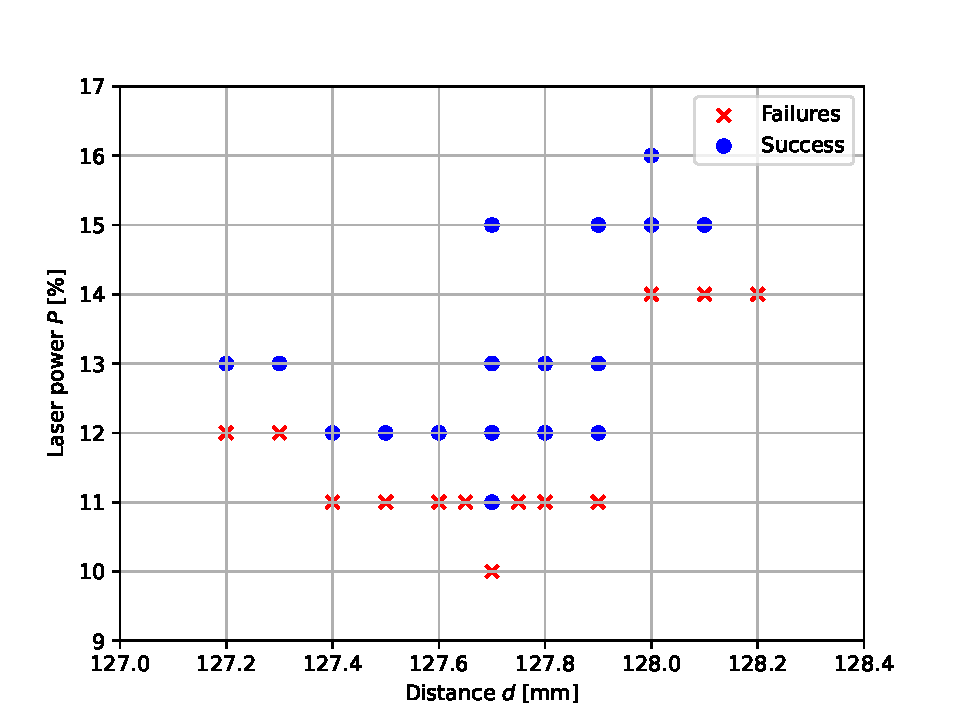
\includegraphics[width=0.75\textwidth]{assets/4 experiments/125mm_focus_threshold.pdf}
                \caption{LSP threshold graph for V1 with \qty{125}{mm} focal length lens}
                \label{fig: 125mm focus threshold}
            \end{figure}
            At power levels lower than 15\%, initiation was unreliable and could take up to 20 attempts to get one initiation. For example, initiation at \qty{11}{\%} was successful once, but it was not possible to repeat this. An even smaller diameter focus was necessary to increase initiation reliability by increasing laser flux at the focus, and a dual-lens system was designed.

            For a dual-lens system, the spot diameter must be calculated numerically. Ray tracing software, such as WinLens3D Basic, calculate the geometry of paraxial \footnote{Rays having small angles and distances to the optical axis} rays and show the path of these rays at the focus. WinLens3D was chosen to simulate the spot size of both the single- and dual-lens systems, as it is free and powerful enough for this application. The modelled lenses are seen in \autoref{fig:modeled lenses}.
            \begin{figure}[!ht]
                \centering
                \begin{subfigure}[t]{0.45\textwidth}
                    \centering
                    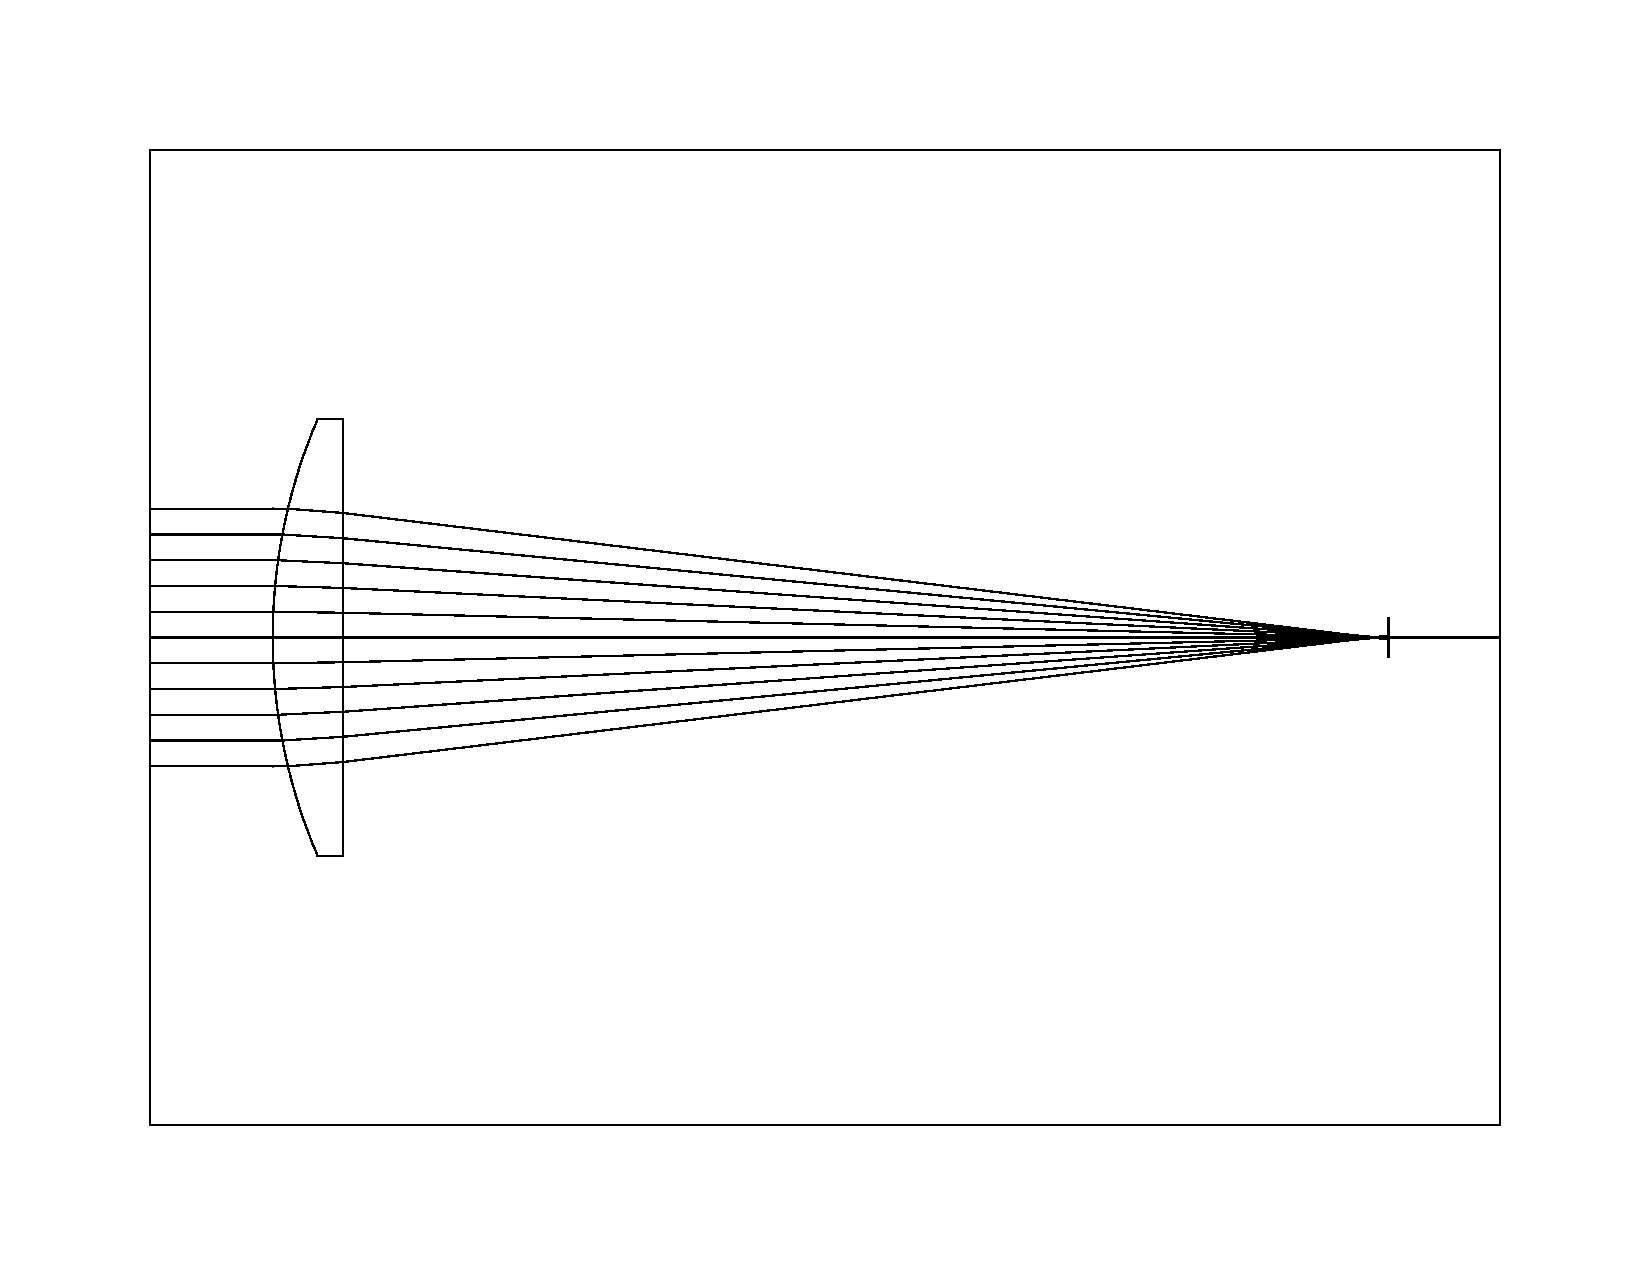
\includegraphics[width=\textwidth]{assets/4 experiments/125lens.pdf}
                    \caption{\qty{125}{mm} focal length lens}
                \end{subfigure}
                \hfill
                \begin{subfigure}[t]{0.45\textwidth}
                    \centering
                    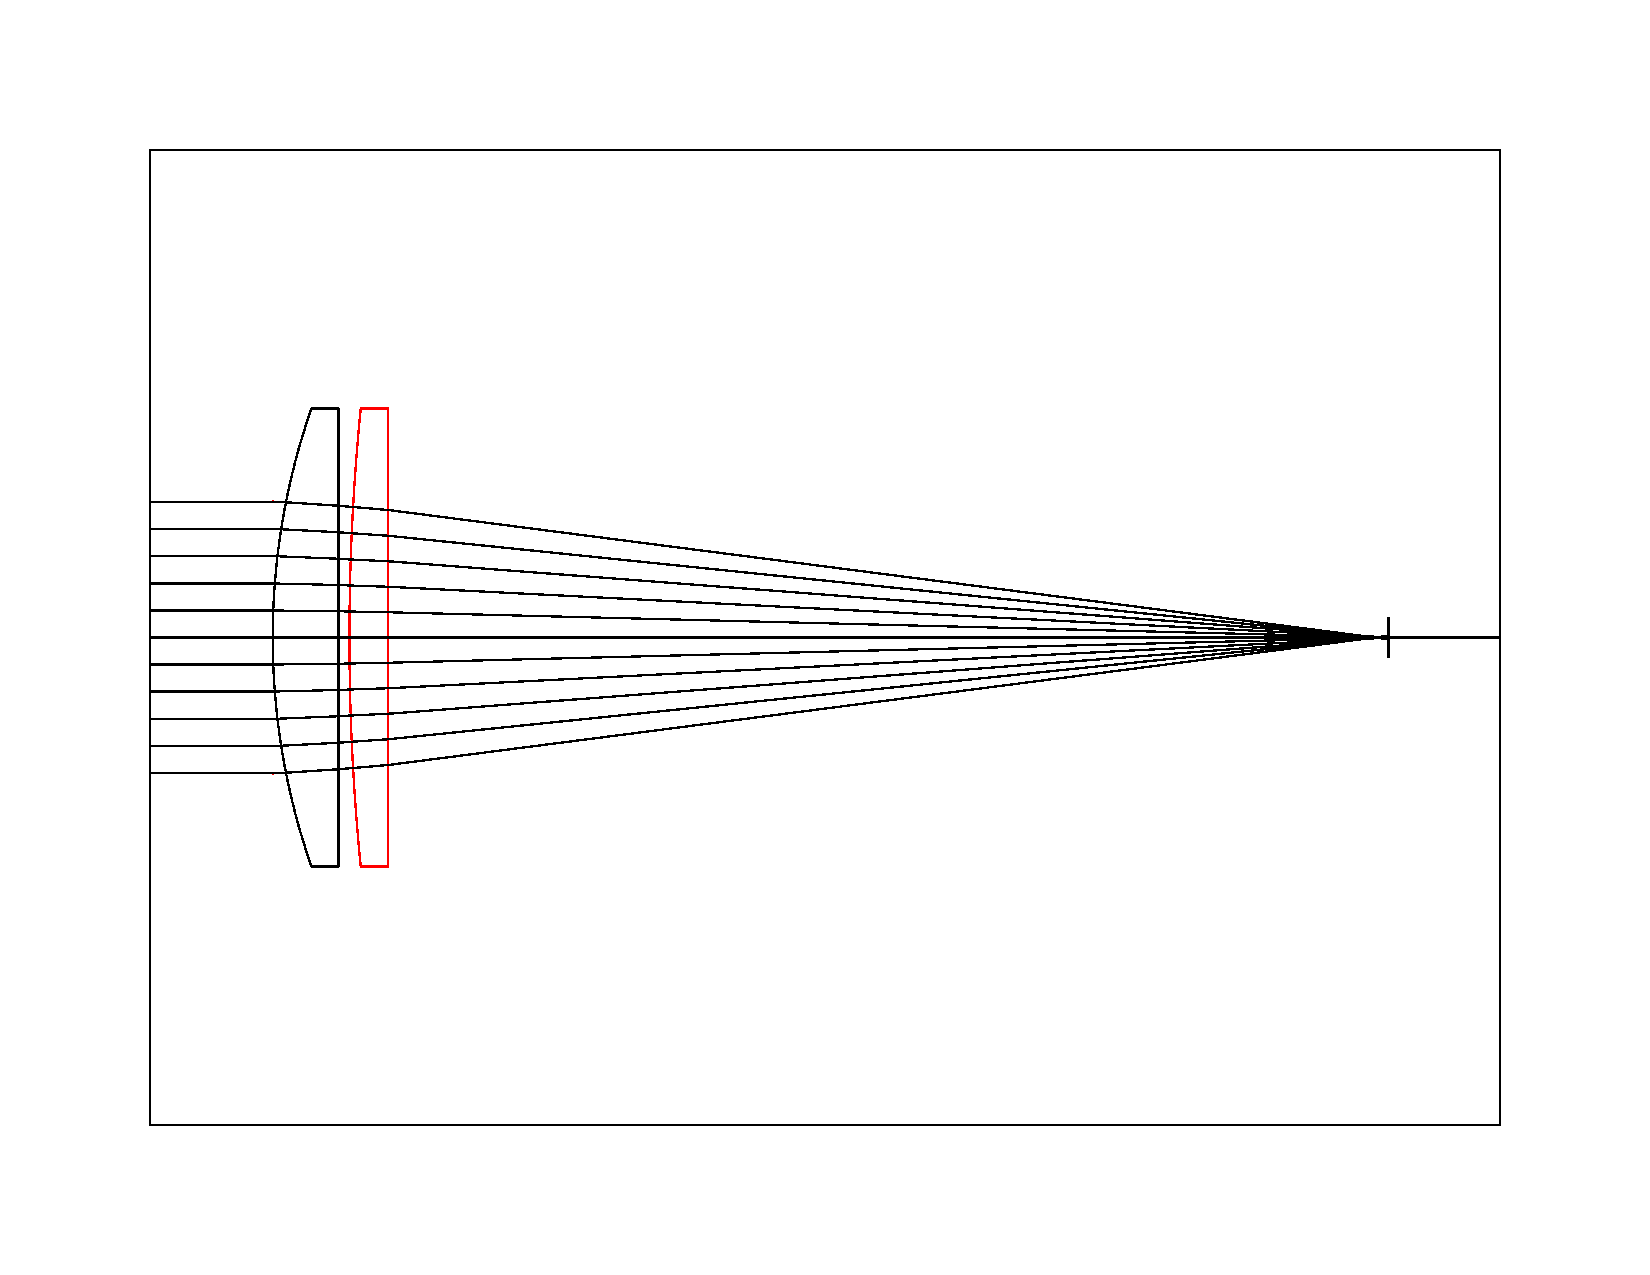
\includegraphics[width=\textwidth]{assets/4 experiments/500 and 150 lenses.pdf}
                    \caption{Dual-lens \qtylist{500;150}{mm} system}
                \end{subfigure}
                \caption{Model of the lenses showing paraxial rays and focus}
                \label{fig:modeled lenses}
            \end{figure}

            With a dual-lens system, the longest focal length lens should be placed first in this case, as the diameter of the beam entering the second lens is maximized. This would lead to a tighter focus, but it was placed after as it was impossible to mount before with the available mounting hardware. The difference in spot size is minimal. A practical consideration for the experiments is that the LSP will be formed upstream of the laser focus when there is no gas flow because the plasma's radiation pre-heats the gas. Therefore, the focus needs to be slightly after the initiation system.

            \autoref{fig:spot diagrams} presents the spot diagrams that were then produced with WinLens3D. Note the difference in scales and spacing used throughout.
            \begin{figure}[!ht]
                \centering
                \begin{subfigure}[t]{\textwidth}
                    \centering
                    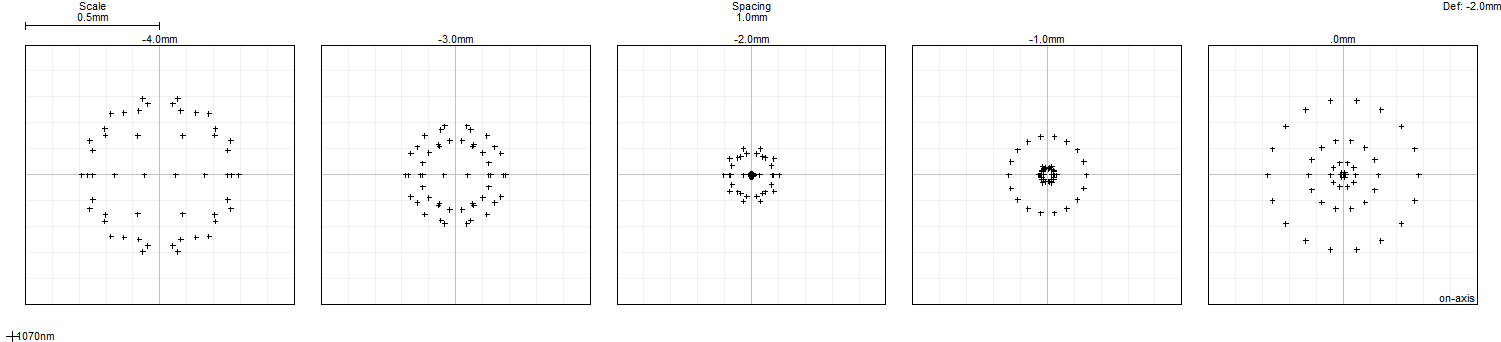
\includegraphics[width=\textwidth]{assets/3 design/100 lens spot diagram.png}
                    \caption{\qty{100}{mm} focal length lens}
                \end{subfigure}
                \begin{subfigure}[t]{\textwidth}
                    \centering
                    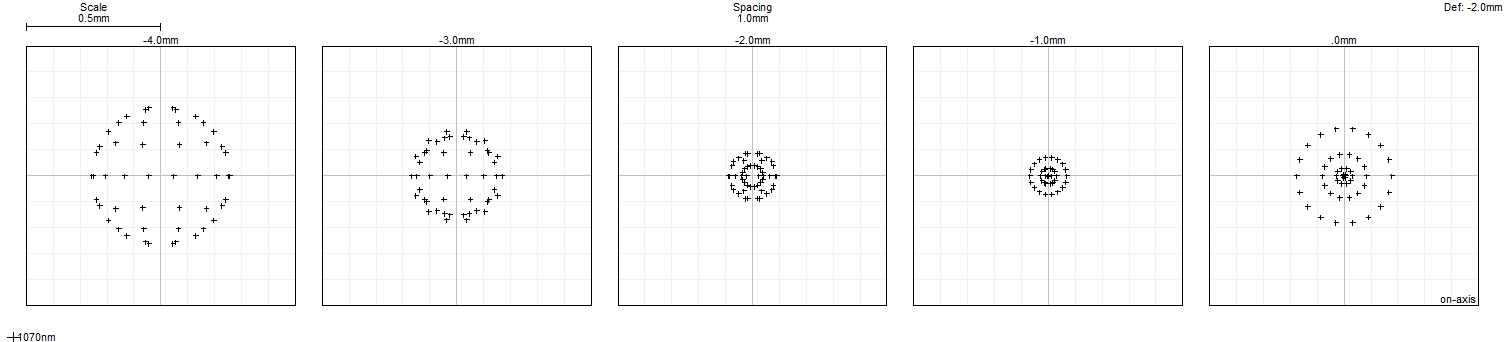
\includegraphics[width=\textwidth]{assets/3 design/125 lens spot diagram.png}
                    \caption{\qty{125}{mm} focal length lens}
                \end{subfigure}
                \begin{subfigure}[t]{\textwidth}
                    \centering
                    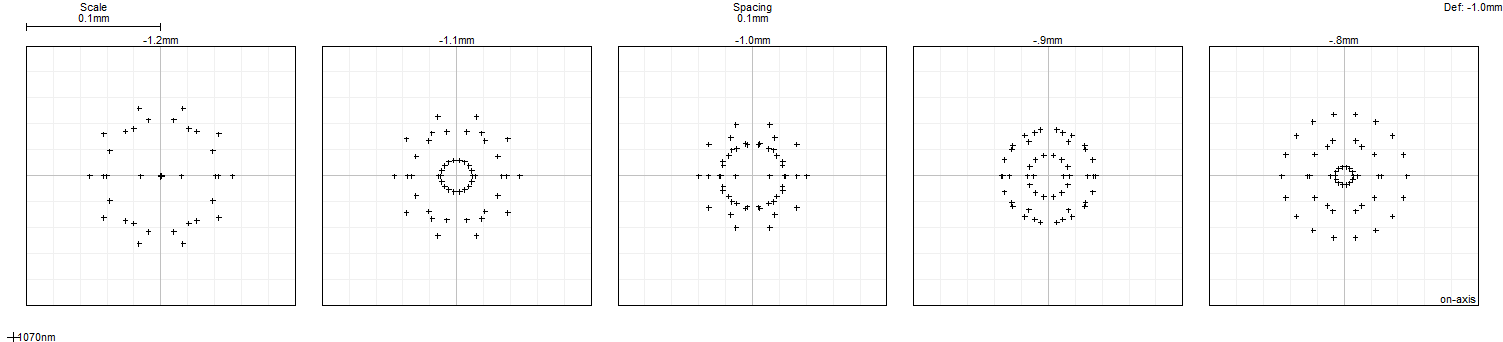
\includegraphics[width=\textwidth]{assets/3 design/500 and 150 lenses spot size.png}
                    \caption{Dual-lens \qtylist{500;150}{mm} system}
                \end{subfigure}
                \caption{Spot diagrams of the three lens systems studied}
                \label{fig:spot diagrams}
            \end{figure}
            From these three spot diagrams, the average laser flux at \qtylist{342}{W} was calculated (see \autoref{tab:laser flux}). It is assumed that the laser energy is evenly distributed in a circle as wide as the farthest ray from the center, which gives a lower bound for the laser flux.
            \begin{table}[!ht]
                \centering
                \caption{Simulated focal length and spot diameter of various lens assemblies in WinLens3D. The average laser flux is calculated for \qty{342}{W} of incident power}
                \label{tab:laser flux}
                \begin{tabularx}{\textwidth}{@{}lX<{\raggedright}X<{\raggedright}X<{\raggedright}X<{\raggedright}@{}}
                \toprule
                Lens & Nominal focal length (\unit{mm}) & Focal length at \qty{1070}{nm} (\unit{mm})& Beam diameter at focus (\unit{mm}) & Average laser flux at \qty{342}{W} (\unit{MW/cm^2}) \\ \midrule
                Single & 125           &  122  &    0.20   &  1.09 \\
                Single & 100           &  93   &    0.15   &  1.94 \\
                Dual & 500, 150      &  110  &    0.08   &  6.80 \\ %calculations for this in C:\Users\gdub5\Documents\WinLens Files
                \bottomrule
                \end{tabularx}
            \end{table}
            The LSP experiments were continued with this dual-lens system (\qty{500}{mm} and \qty{150}{mm} focal lengths), as it offers a 6.25 times increase of the laser flux compared to the single \qtylist{125}{mm} focal length lens. To increase the laser flux even more, an aspheric lens of comparable focal length could be used, though it costs 10 times as much as a single plano-convex lens. \autoref{fig:V1 dual-lens threshold graph} presents a record of LSP initiation attempts at various power settings and lens axial positions with this dual-lens system in V1.
            \begin{figure}[!ht]
                \centering
                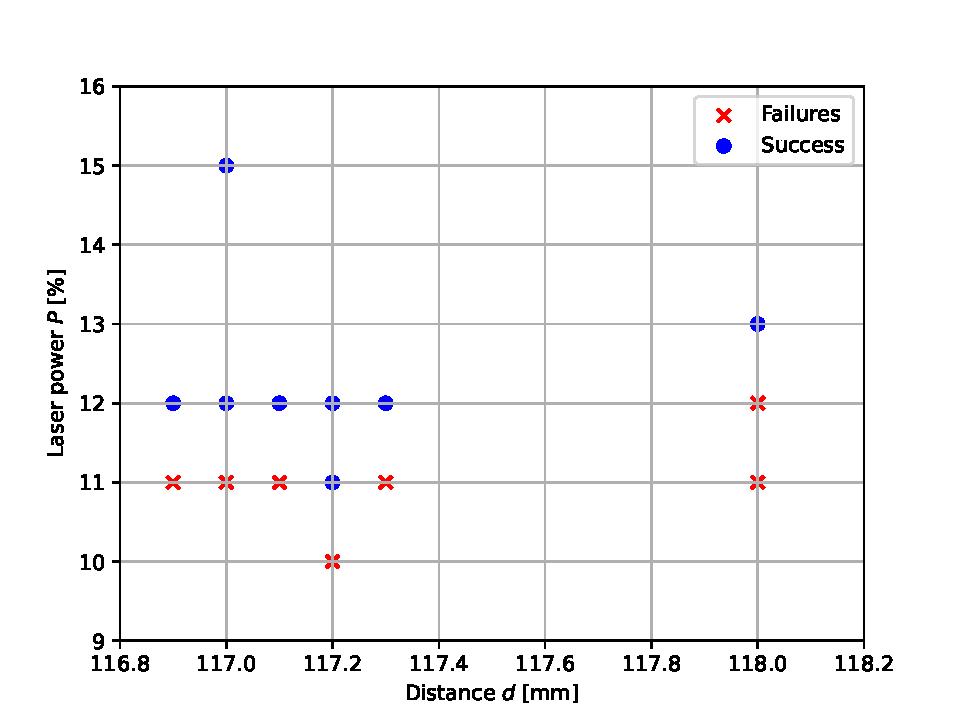
\includegraphics[width=0.75\textwidth]{assets/4 experiments/duallens_focus_threshold.pdf}
                \caption{LSP threshold graph for V1 with dual-lens system}
                \label{fig:V1 dual-lens threshold graph}
            \end{figure}
            The completion of these tests validated the dual-lens design, showing that LSPs in the CW power regime of the laser could be generated. The first LSPs in V2 were therefore done using the dual-lens system. A similar graph to \autoref{fig:V1 dual-lens threshold graph} was then created with V2 to find the lens position where the minimum laser power could reliably initiate QCW LSP. \autoref{fig:V2 threshold graph} presents these initiation attempts.
            \begin{figure}[!ht]
                \centering
                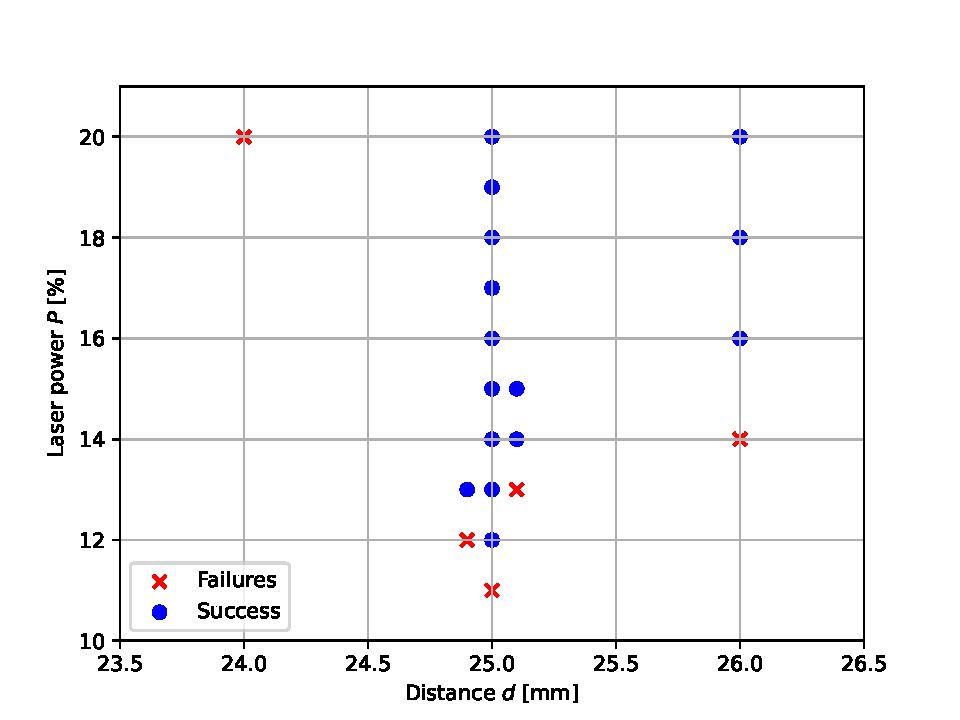
\includegraphics[width=0.75\textwidth]{assets/4 experiments/V2_focus_threshold.pdf}
                \caption{LSP threshold graph for V2 with dual-lens system}
                \label{fig:V2 threshold graph}
            \end{figure}

        \subsection{V2 CW LSP}

            A \qty{100}{\%} power CW shot was then attempted with static argon at \qty{20}{bar}. 

            \begin{figure}[h]
    \centering
    \begin{subfigure}[t]{0.3\textwidth}
        \centering
        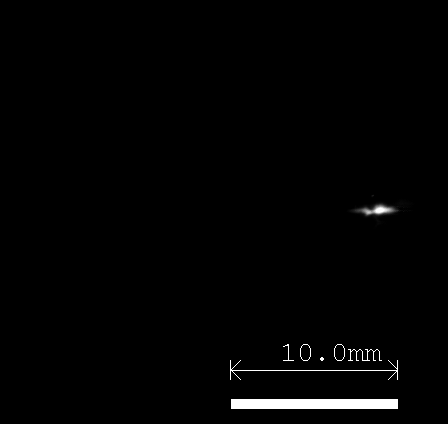
\includegraphics[width=\textwidth]{assets/4 experiments/V1 Spark Ignition Frames/LSP142_SPRK15_Fr32.bmp}
        \caption{\qty{3.2}{ms}}
        %\label{fig:V1_ignition_frames_16}
    \end{subfigure}
    \hfill
    \begin{subfigure}[t]{0.3\textwidth}
        \centering
        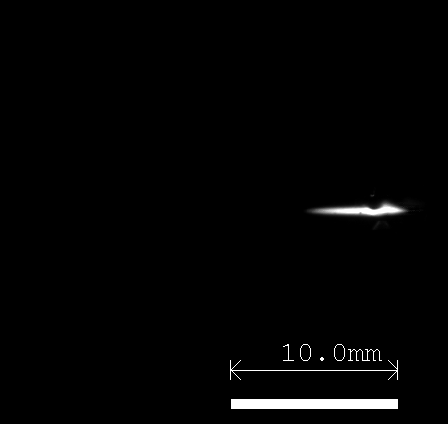
\includegraphics[width=\textwidth]{assets/4 experiments/V1 Spark Ignition Frames/LSP142_SPRK15_Fr33.bmp}
        \caption{\qty{3.3}{ms}}
        %\label{fig:ignition_frames_17}
    \end{subfigure}
    \hfill
    \begin{subfigure}[t]{0.3\textwidth}
        \centering
        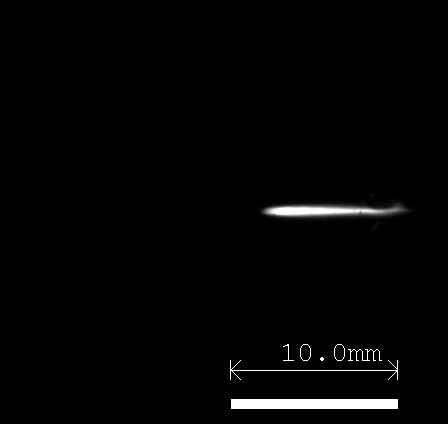
\includegraphics[width=\textwidth]{assets/4 experiments/V1 Spark Ignition Frames/LSP142_SPRK15_Fr35.bmp}
        \caption{\qty{3.5}{ms}}
        %\label{fig:ignition_frames_18}
    \end{subfigure}
    \begin{subfigure}[t]{0.3\textwidth}
        \centering
        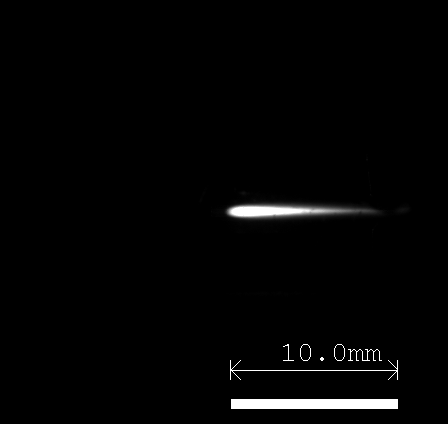
\includegraphics[width=\textwidth]{assets/4 experiments/V1 Spark Ignition Frames/LSP142_SPRK15_Fr38.bmp}
        \caption{\qty{3.8}{ms}}
        %\label{fig:ignition_frames_19}
    \end{subfigure}
    \hfill
    \begin{subfigure}[t]{0.3\textwidth}
        \centering
        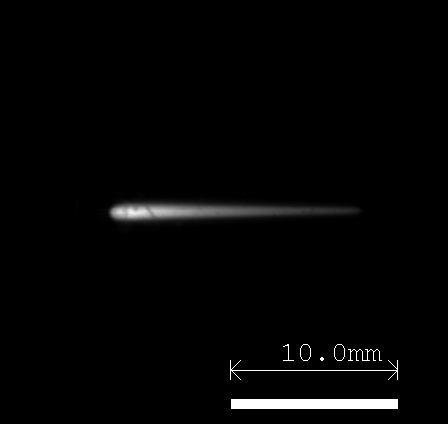
\includegraphics[width=\textwidth]{assets/4 experiments/V1 Spark Ignition Frames/LSP142_SPRK15_Fr69.bmp}
        \caption{\qty{6.9}{ms}}
        %\label{fig:ignition_frames_20}
    \end{subfigure}
    \hfill
    \begin{subfigure}[t]{0.3\textwidth}
        \centering
        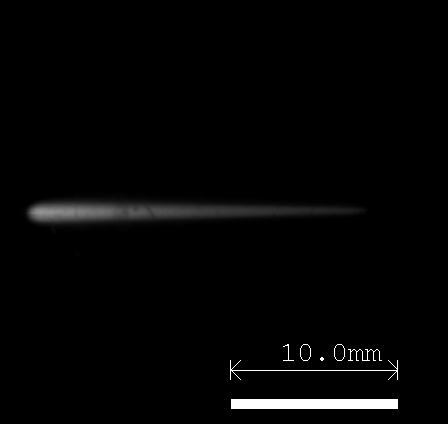
\includegraphics[width=\textwidth]{assets/4 experiments/V1 Spark Ignition Frames/LSP142_SPRK15_Fr130.bmp}
        \caption{\qty{13.0}{ms}}
        %\label{fig:ignition_frames_21}
    \end{subfigure}
    \caption{LSP spark initiation: \qty{3080}{W}, \qty{20}{bar}. \shotsettings{LSP142\_SPRK15}{0.1?? CHANGE}{22}{2048}}
    \label{fig:V1_spark_initiation_frames}
\end{figure}

            The webcam footage (\autoref{fig:CW_V2_webcam_frames}) will be examined first. The laser is first turned on. A flash marks the spark initiation and lifetime of the LSP. This flash lasts only a few frames. Notice the higher brightness in \autoref{fig:CW_V2_webcam_frames_LSP}, reflecting off various surfaces like the white box (PCB signal conditioner) on the left of the collimator. The laser was kept running for about a second before it was turned off.

            \begin{figure}[h]
    \centering
    \begin{subfigure}[t]{0.3\textwidth}
        \centering
        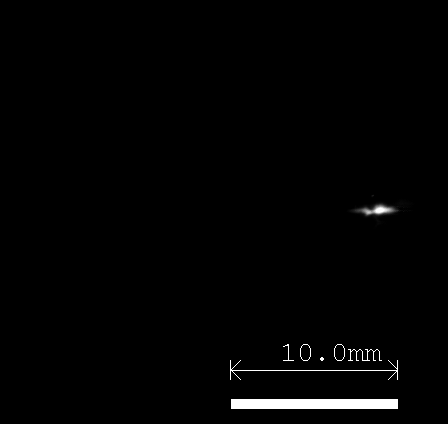
\includegraphics[width=\textwidth]{assets/4 experiments/V1 Spark Ignition Frames/LSP142_SPRK15_Fr32.bmp}
        \caption{\qty{3.2}{ms}}
        %\label{fig:V1_ignition_frames_16}
    \end{subfigure}
    \hfill
    \begin{subfigure}[t]{0.3\textwidth}
        \centering
        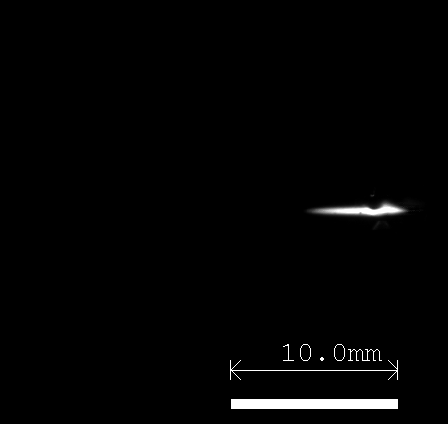
\includegraphics[width=\textwidth]{assets/4 experiments/V1 Spark Ignition Frames/LSP142_SPRK15_Fr33.bmp}
        \caption{\qty{3.3}{ms}}
        %\label{fig:ignition_frames_17}
    \end{subfigure}
    \hfill
    \begin{subfigure}[t]{0.3\textwidth}
        \centering
        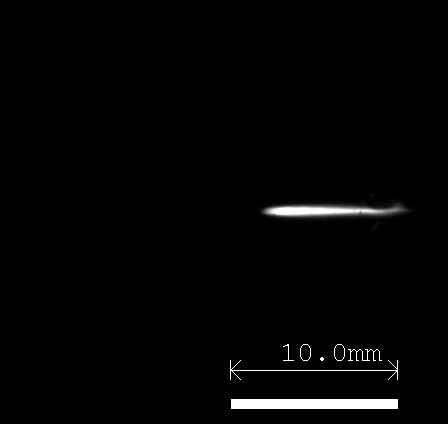
\includegraphics[width=\textwidth]{assets/4 experiments/V1 Spark Ignition Frames/LSP142_SPRK15_Fr35.bmp}
        \caption{\qty{3.5}{ms}}
        %\label{fig:ignition_frames_18}
    \end{subfigure}
    \begin{subfigure}[t]{0.3\textwidth}
        \centering
        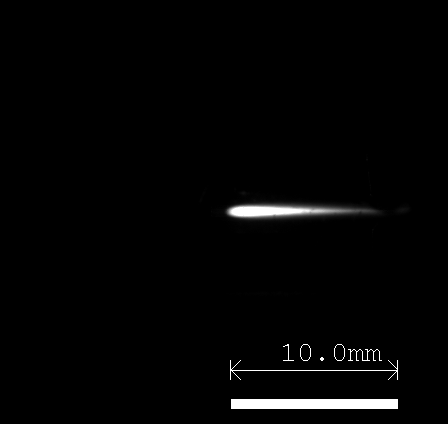
\includegraphics[width=\textwidth]{assets/4 experiments/V1 Spark Ignition Frames/LSP142_SPRK15_Fr38.bmp}
        \caption{\qty{3.8}{ms}}
        %\label{fig:ignition_frames_19}
    \end{subfigure}
    \hfill
    \begin{subfigure}[t]{0.3\textwidth}
        \centering
        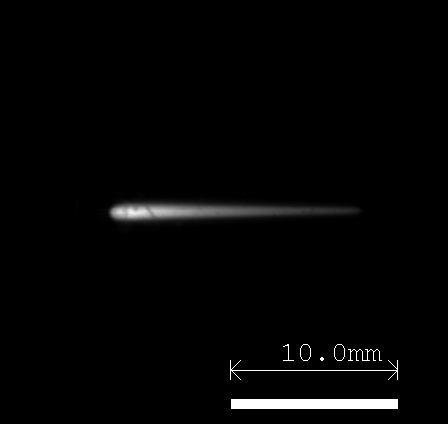
\includegraphics[width=\textwidth]{assets/4 experiments/V1 Spark Ignition Frames/LSP142_SPRK15_Fr69.bmp}
        \caption{\qty{6.9}{ms}}
        %\label{fig:ignition_frames_20}
    \end{subfigure}
    \hfill
    \begin{subfigure}[t]{0.3\textwidth}
        \centering
        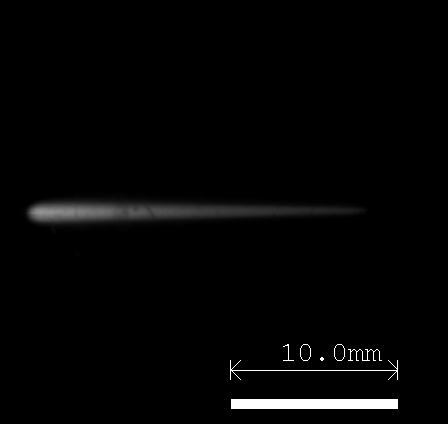
\includegraphics[width=\textwidth]{assets/4 experiments/V1 Spark Ignition Frames/LSP142_SPRK15_Fr130.bmp}
        \caption{\qty{13.0}{ms}}
        %\label{fig:ignition_frames_21}
    \end{subfigure}
    \caption{LSP spark initiation: \qty{3080}{W}, \qty{20}{bar}. \shotsettings{LSP142\_SPRK15}{0.1?? CHANGE}{22}{2048}}
    \label{fig:V1_spark_initiation_frames}
\end{figure}

            Observation of the high-speed camera footage (\autoref{fig:CW_V2_Photron_frames}), recorded at 10,000 frames per second, showed the CW LSP starting at frame 32 (\qty{3.2}{ms}) and ending at frame 883 (\qty{88.3}{ms}), lasting \qty{85.1}{ms}. This represents a 1.7 times longer lifetime than the maximum QCW pulse length of \qty{50.0}{ms} at this power. The brightness of the plasma increases regularly after initiation, to reach its maximum intensity around \qty{50}{ms}. The maximum brightness is constant for \qty{10}{ms}. A flickering of the LSP is seen at \qty{70.0}{ms}, before it died down and was completely extinguished after \qty{88.3}{ms}. This was the first CW LSP generated in the lab.

            \begin{figure}[!ht]
                \centering
                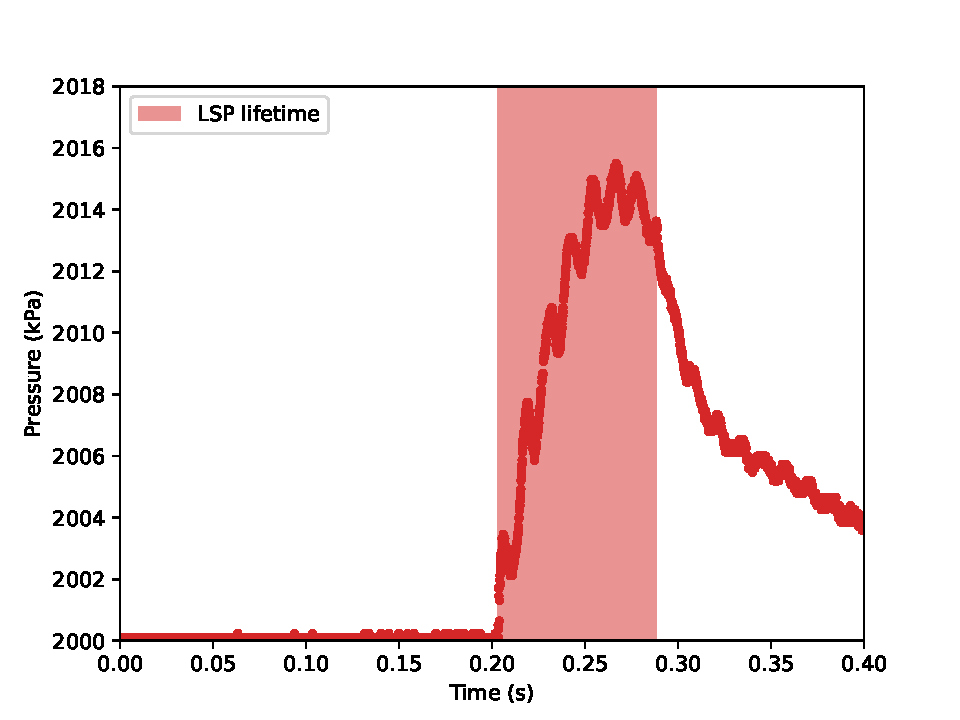
\includegraphics[width=0.75\textwidth]{assets/4 experiments/CW pressure rise.pdf}
                \caption{Dynamic pressure rise from CW LSP measured with PCB transducer}
                \label{fig:CW pressure rise}
            \end{figure}

            \autoref{fig:CW pressure rise} shows the pressure rise recorded by the PCB transducer connected to the oscilloscope. Minimal damage to the window was noticed after this test.

        % \subsection{CW power measurement}

        %     Wanted to see where exactly the pulsed power threshold was. For this, needed a max CW power measurement to compare against. 
    
        %     Tried to measure max CW power through two lenses, without the V2 apparatus. The two lenses were rated for this flux, but the 500 mm focal length lens shattered after about \qty{50}{s} of CW lasing. The leading hypothesis is that as the lens' temperature increased, it expanded, shattering it
    
        %     [graph of laser power that broke lens]
    
        %     \begin{figure}[!ht]
        %         \centering
        %         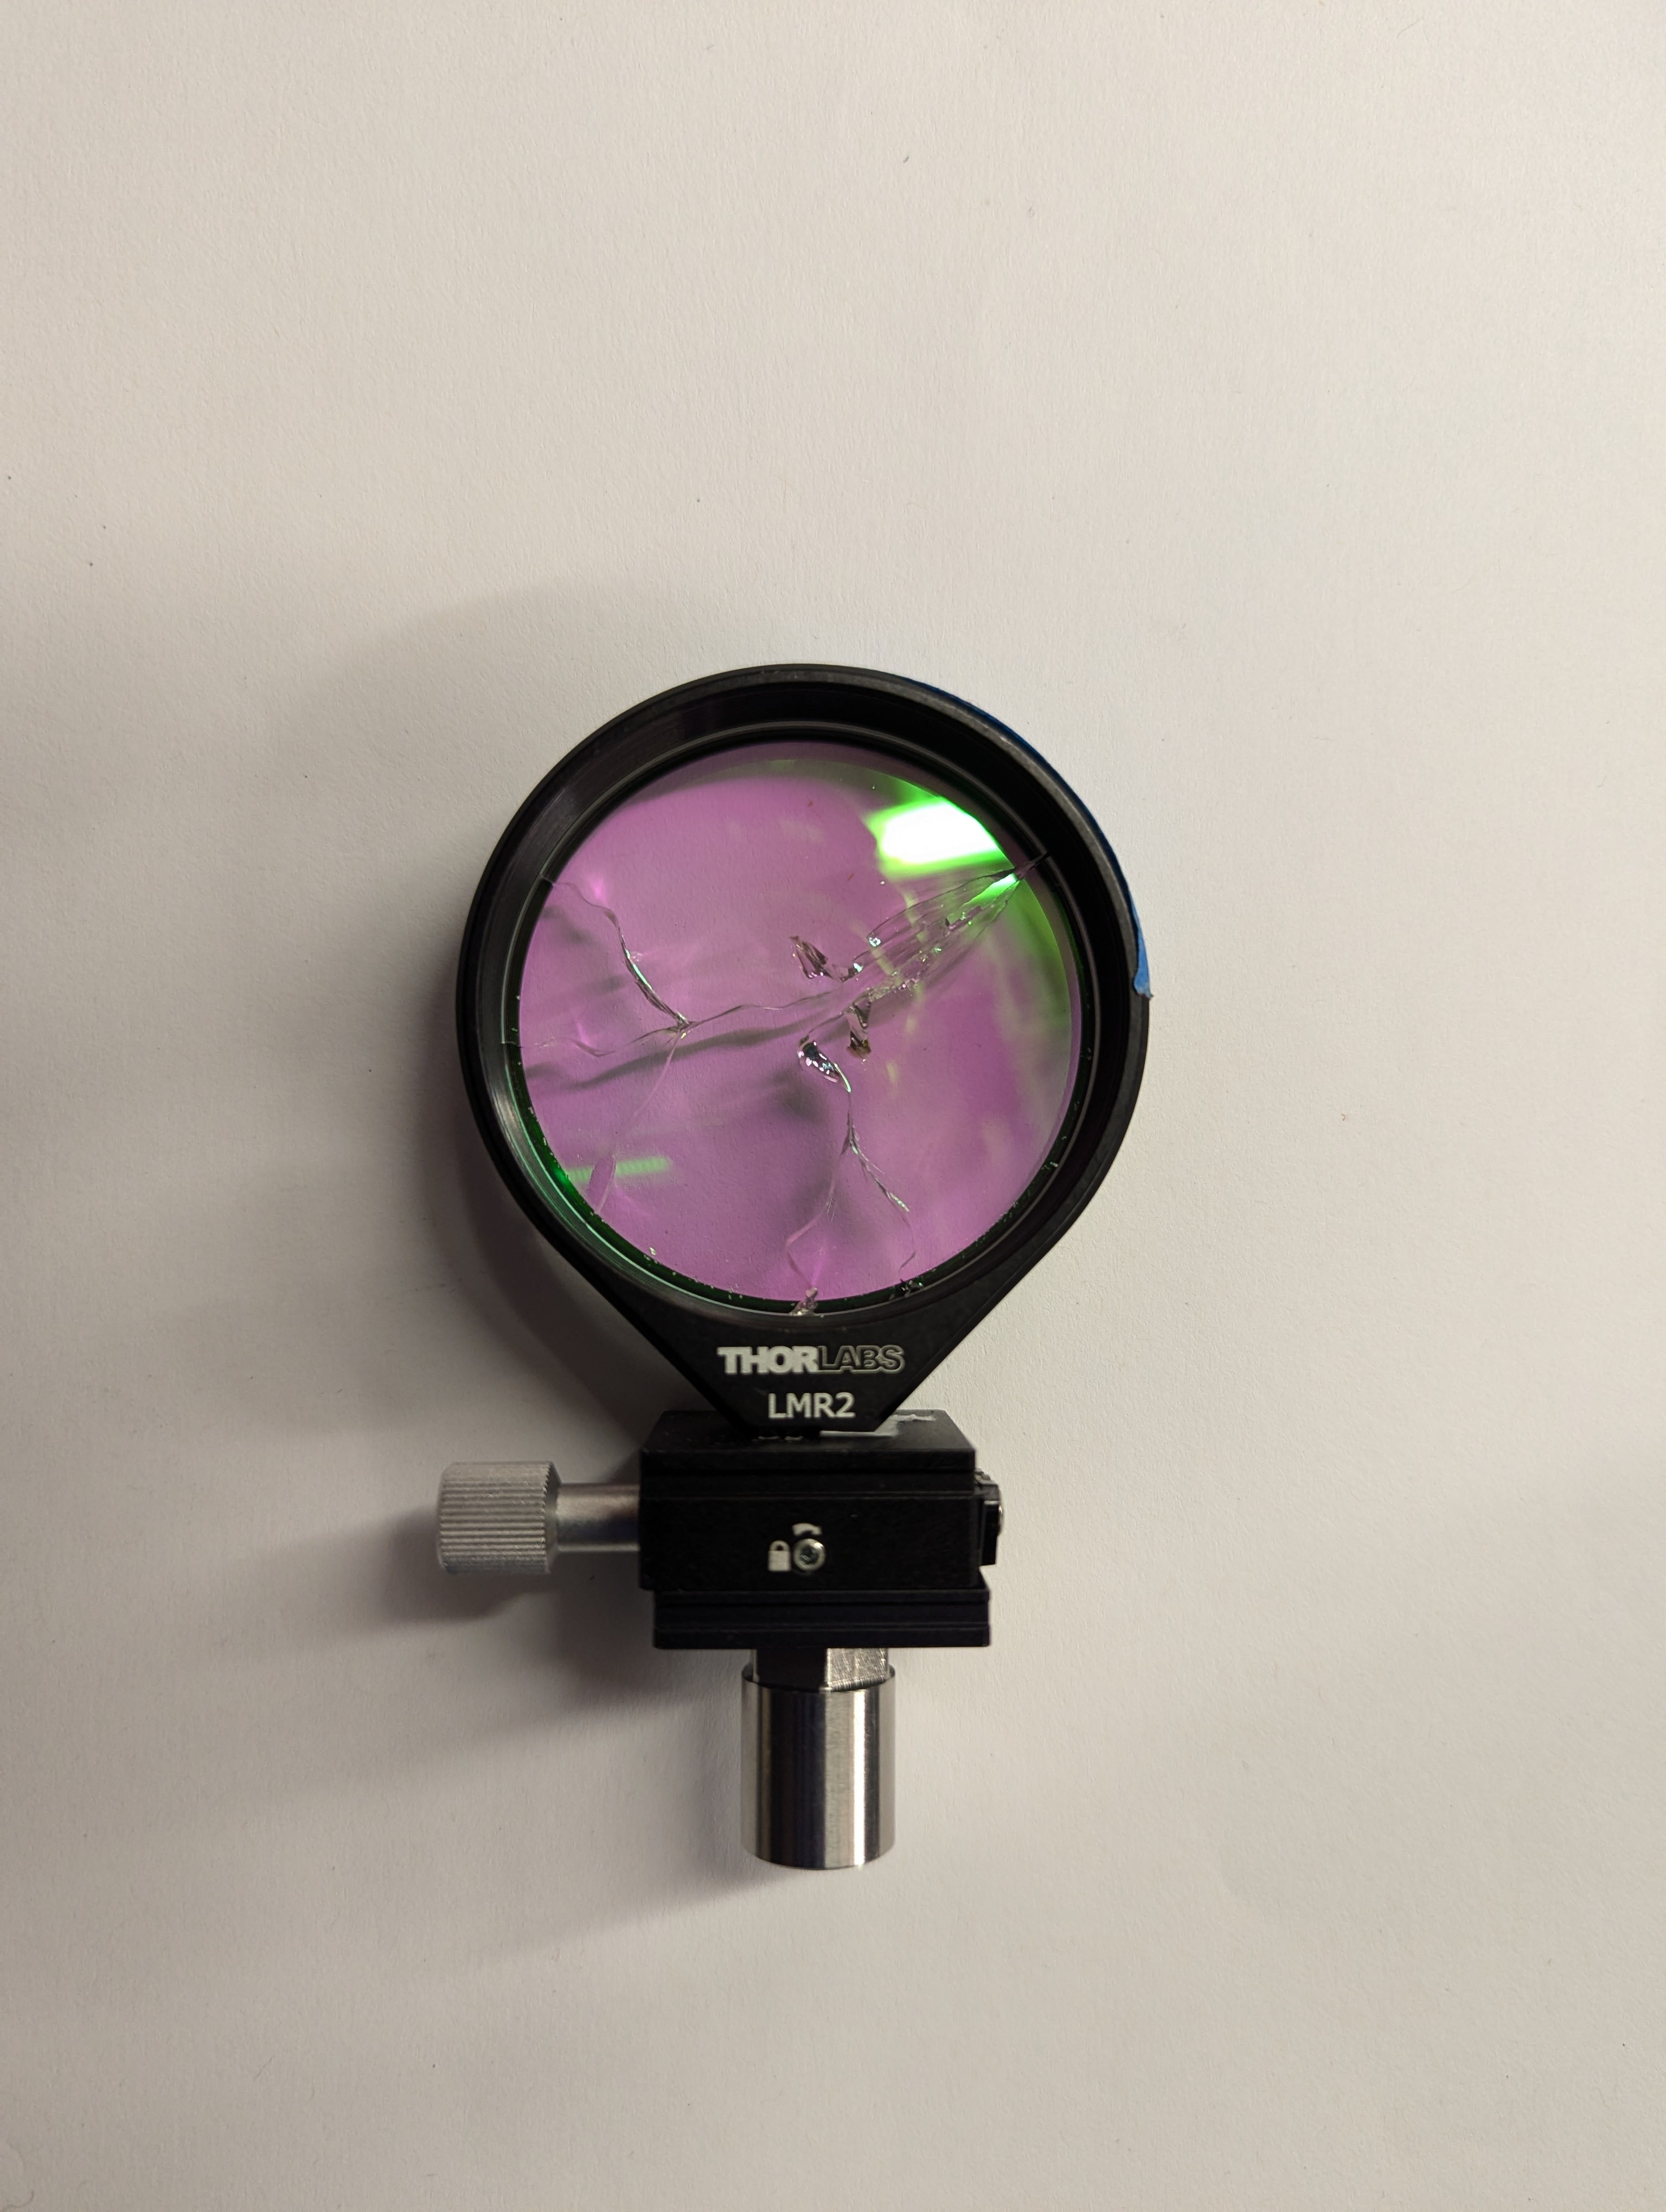
\includegraphics[width=0.25\textwidth]{assets/4 experiments/Shattered 500 mm lens.jpg}
        %         \caption{Shattered \qty{500}{mm} focal length lens}
        %     \end{figure}
    
        %     This test showed a \qty{314}{W} max CW power.
    
        %     Therefore, future CW tests will have to stay under this maximum time period, unless a lens cooling system is implemented. This could be as simple as a fan blowing cool air onto the lens.

        %     \todo{Long duration lasing test: determine limits of V2 under max CW power: conclusion: lens cracked due to expansion. No optical damage of the glass was seen}

        % \subsection{Summary of results}

        %     \begin{table}[!ht]
        %         \centering
        %         \caption{Summary of the static LSP validation campaign}
        %         \label{tab:validation}
        %         \begin{tabular}{@{}lll@{}}
        %         \toprule
        %         Validation Question               & Yes & No \\ \midrule
        %         Is LSP spark initiation possible? & X   &    \\
        %         Is QCW LSP possible in V2?        & X   &    \\
        %         Is CW LSP possible in V2?         & X   &   
        %         \end{tabular}
        %     \end{table}


    \section{V2 Cold flow thruster characterization}

        \subsection{Cold flow thrust tests}

            Cold flow tests (laser off) were completed with V2 to give a baseline measurement of thrust before eventual hot fire tests (laser on), and to validate the functioning of all data acquisition systems.

            For thrust tests, pressure and thrust were recorded. \autoref{fig:20bar cold flow} shows a typical thrust and pressure curve for a chamber pressure of \qty{20}{bar}. Note that the thrust measurement does not return to the same value it was at initially.

            \begin{figure}[!ht]
                \centering
                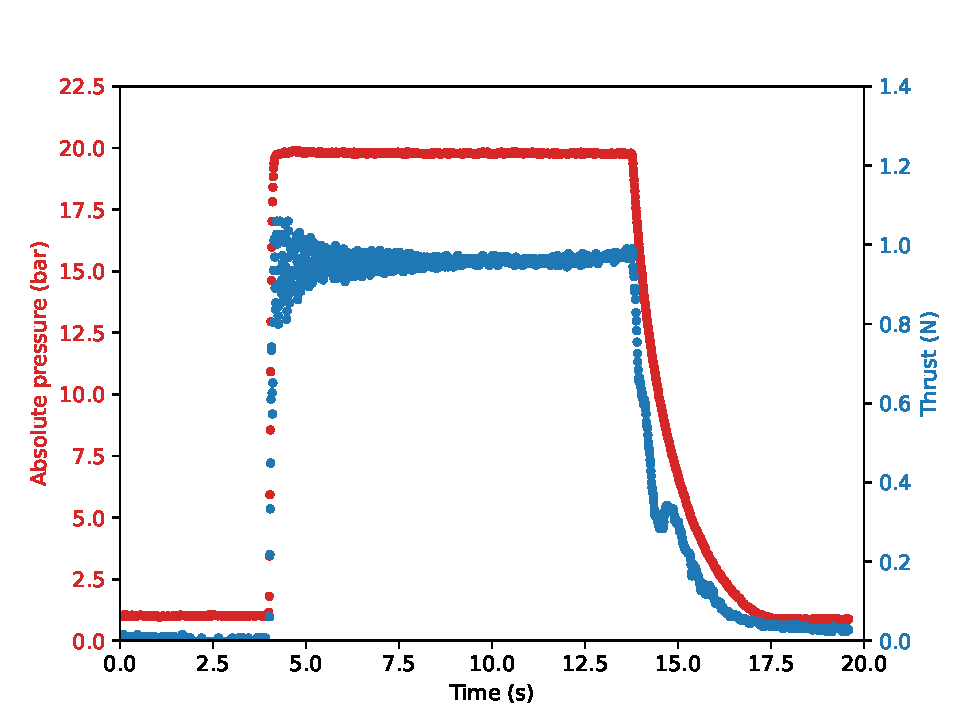
\includegraphics[width=0.75\textwidth]{assets/4 experiments/Example thrust 20 bar.pdf}
                \caption{Typical cold flow pressure and thrust curves for 20 bar chamber pressure}
                \label{fig:20bar cold flow}
            \end{figure}

            Next, cold flow thrust tests were completed at chamber pressures from \qtyrange{5}{35}{bar}. A linear curve fit of the experimental results is presented in \autoref{fig:coldflow pressure-thrust}.

            \begin{figure}[!ht]
                \centering
                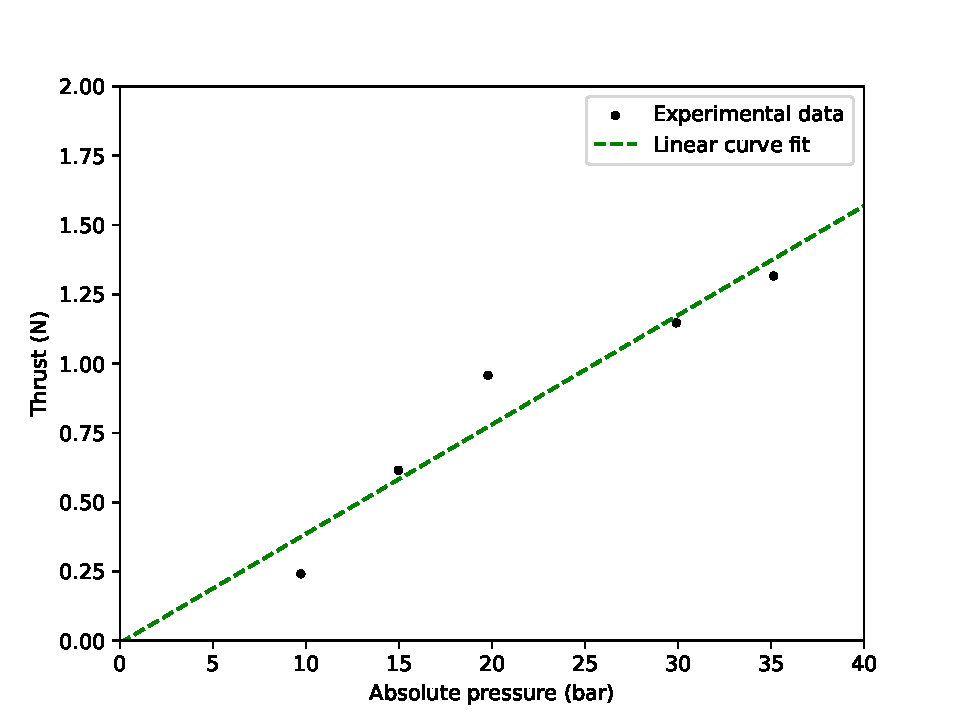
\includegraphics[width=0.75\textwidth]{assets/4 experiments/pressure-thrust graph.pdf}
                \caption{Absolute pressure versus thrust and curve fit of pressure-thrust relation}
                \label{fig:coldflow pressure-thrust}
            \end{figure}

            The empirical relation of pressure versus thrust is given by:
            \[
            \text{Thrust (N)} = 0.0394*\text{Pressure (bar)} + 0.0318
            \]

            Repeatability of the thrust measurements was then examined with the Honeywell FSG005WNPB \qtyrange{0}{5}{N} load cell and a \qty{200}{g} preload, with an argon inlet pressure of \qty{20}{bar}. The raw voltage of the load cell was recorded, as the hysteresis was the point of interest and not the thrust.
            \begin{figure}[h]
                \centering
                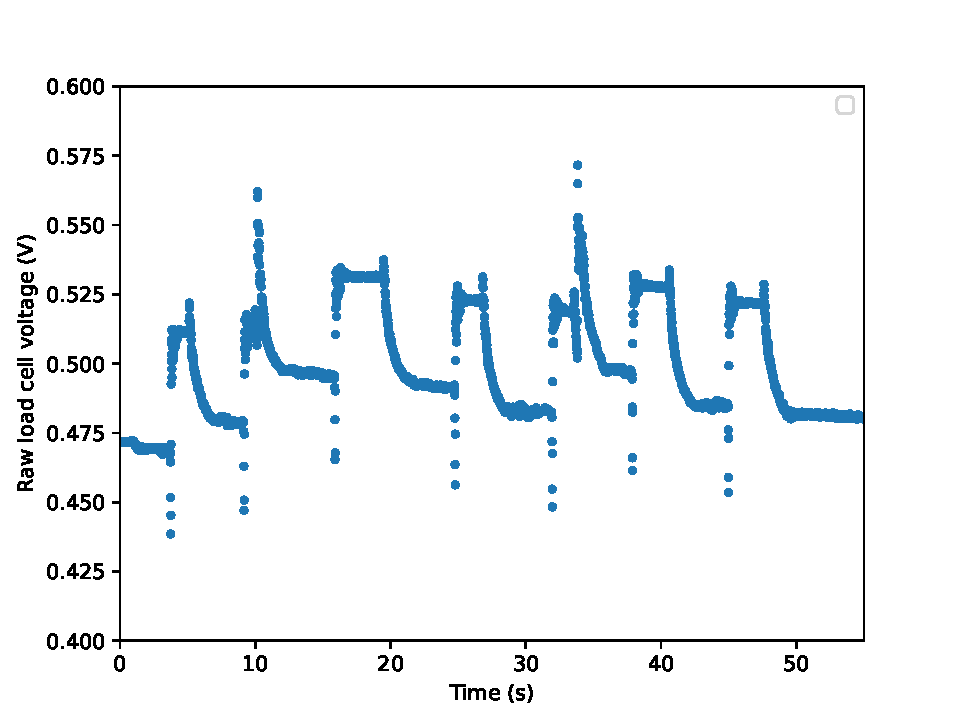
\includegraphics[width=0.75\textwidth]{assets/4 experiments/hysterisis graph.pdf}
                \caption{Multiple cold flow thrust tests in succession}
                \label{fig:hysteresis}
            \end{figure}
            Significant hysteresis of the thrust stand is seen in \autoref{fig:hysteresis}. The final thrust was sometimes higher than the initial thrust, sometimes lower. The discontinuities at \qtylist{10;35}{s} were due to the accidental shutoff of the gas supply.

        \subsection{Thruster nozzle effective sonic area $A^*$}

            To determine the mass flow rate $\dot{m}$ of the thruster, sonic isentropic flow at the nozzle throat was assumed. The following equation can then be used:
            \begin{equation}
                \dot{m} = \frac{A^* p}{\sqrt{T}}\sqrt{\frac{\gamma}{R}}\left(\frac{\gamma + 1}{2}\right)^{\frac{-\gamma + 1}{2(\gamma-1)}}
            \end{equation}
            Where $A^*$, the nozzle effective sonic area, is an unknown, $p$ is pressure, $T$ is temperature, $\gamma$ is the specific heat ratio, and $R$ is the gas constant.
        
            To characterize the effective sonic area, $A^*$, of the thruster nozzle, a choked orifice blow-down test was done based upon the theory in \textcite{saadCompressibleFluidFlow}. V2 in flowing configuration was pressurized to \qty{20}{bar} of argon. The argon flow was then closed. The pressure curve was recorded by the Omega transducer.

            The internal volume of the V2 thruster in flowing configuration was determined by weighing it before and after it was filled with isopropyl alcohol. Using a density of \qty{785}{kg/m^3}, the volume was found to be \qty{9.68e-6}{m^3}, or \qty{9.68}{ml}.

            The following expression for the pressure-time history of a blow down choked orifice flow \cite{saadCompressibleFluidFlow} was then implemented in Python. As the timescale is short (less than 10 seconds), the process is considered adiabatic, and the isentropic case is used:

            \begin{equation}
                t =  \frac{-2V \left[\left(\frac{p(t)}{p_i}\right)^{(1-\gamma) / 2\gamma}\right]}{(1-\gamma) R \sqrt{T} A \sqrt{\frac{\gamma}{R}(\frac{2}{\gamma + 1})^{(\gamma+1) / (\gamma-1)}}}
            \end{equation}

            Where $t$ is time, $p(t)$ is the absolute pressure in the system at time $t$, $p_i$ is the initial absolute pressure in the system, $V$ is the volume of the V2 thruster and tubing after the valve, $T$ is temperature, $A$ is the area of the nozzle's throat. With this equation, the absolute pressure in bar was plotted versus time in seconds for different values of $A$, with a specific heat ratio $\gamma$ of 1.67, a temperature of \qty{300}{K}, and an R of \qty{208.13}{J/kg*K} (see \autoref{fig:saad blowdown}). An experimental pressure curve was also overlaid, similar to \autoref{fig:20bar cold flow}, but cut to only show the decrease in pressure right after the gas feed valve is closed. The time at which this valve is closed is defined as $t=0$.

            \begin{figure}[!ht]
                \centering
                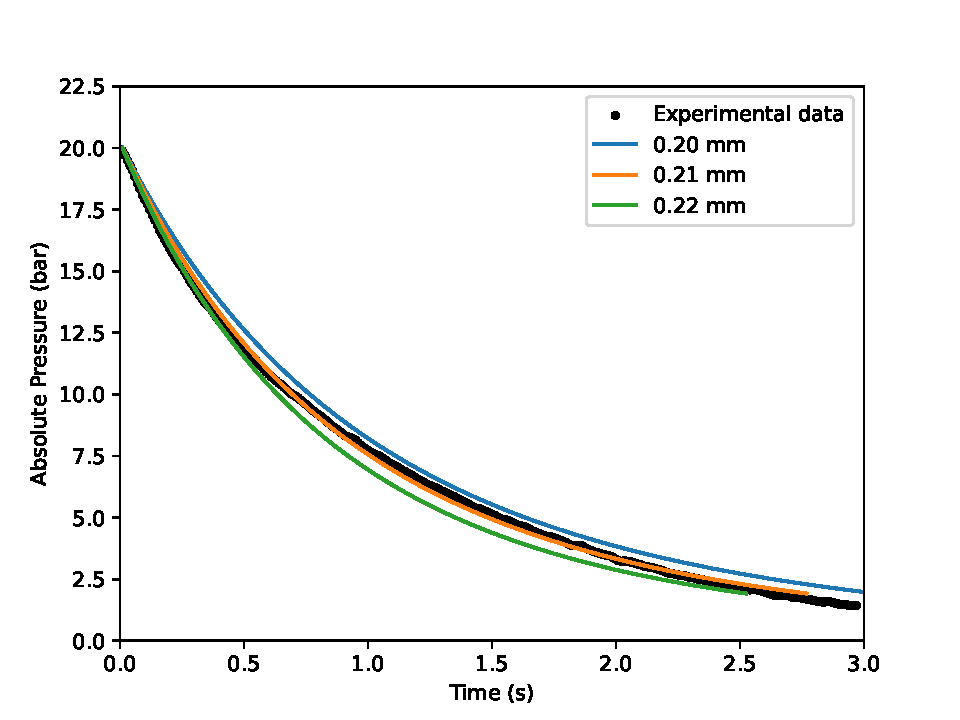
\includegraphics[width=0.75\textwidth]{assets/4 experiments/Saad blowdown fit.pdf}
                \caption{Saad blowdown model and experimental data}
                \label{fig:saad blowdown}
            \end{figure}

            The best match was found to be an area of \qty{3.46e-8}{m^2}, giving a nozzle diameter of \qty{0.21}{mm}.

        \subsection{Needle valve effective sonic area $A^*$}

            The WL14H-320P needle valve (see \autoref{fig:Needle valve}) \todo{?? Links to design chapter} was calibrated to relate its rotation increments to its flow rate. This was undertaken by connecting the valve's input to a gas supply, while the valve's output was connected to a bubble flow meter constructed for this experiment (\autoref{fig:bubble meter}). The bubble flow meter and experiment methodology were presented in \textcite{barigouFluidMechanicsSoap1993}.

            A uniform bubble created at the base of the tube rises upwards towards the top of the tube as it is displaced by the pressurizing gas. This end of the tube is open to the atmosphere. A stopwatch is started when the bubble passes the base of the green tape line and stopped once the bubble passes the base of the red tape line. These stopwatch measurements are repeated three times and averaged. This enables precise measurement of the volumetric flow rate.

            \begin{figure}[!ht]
                \centering
                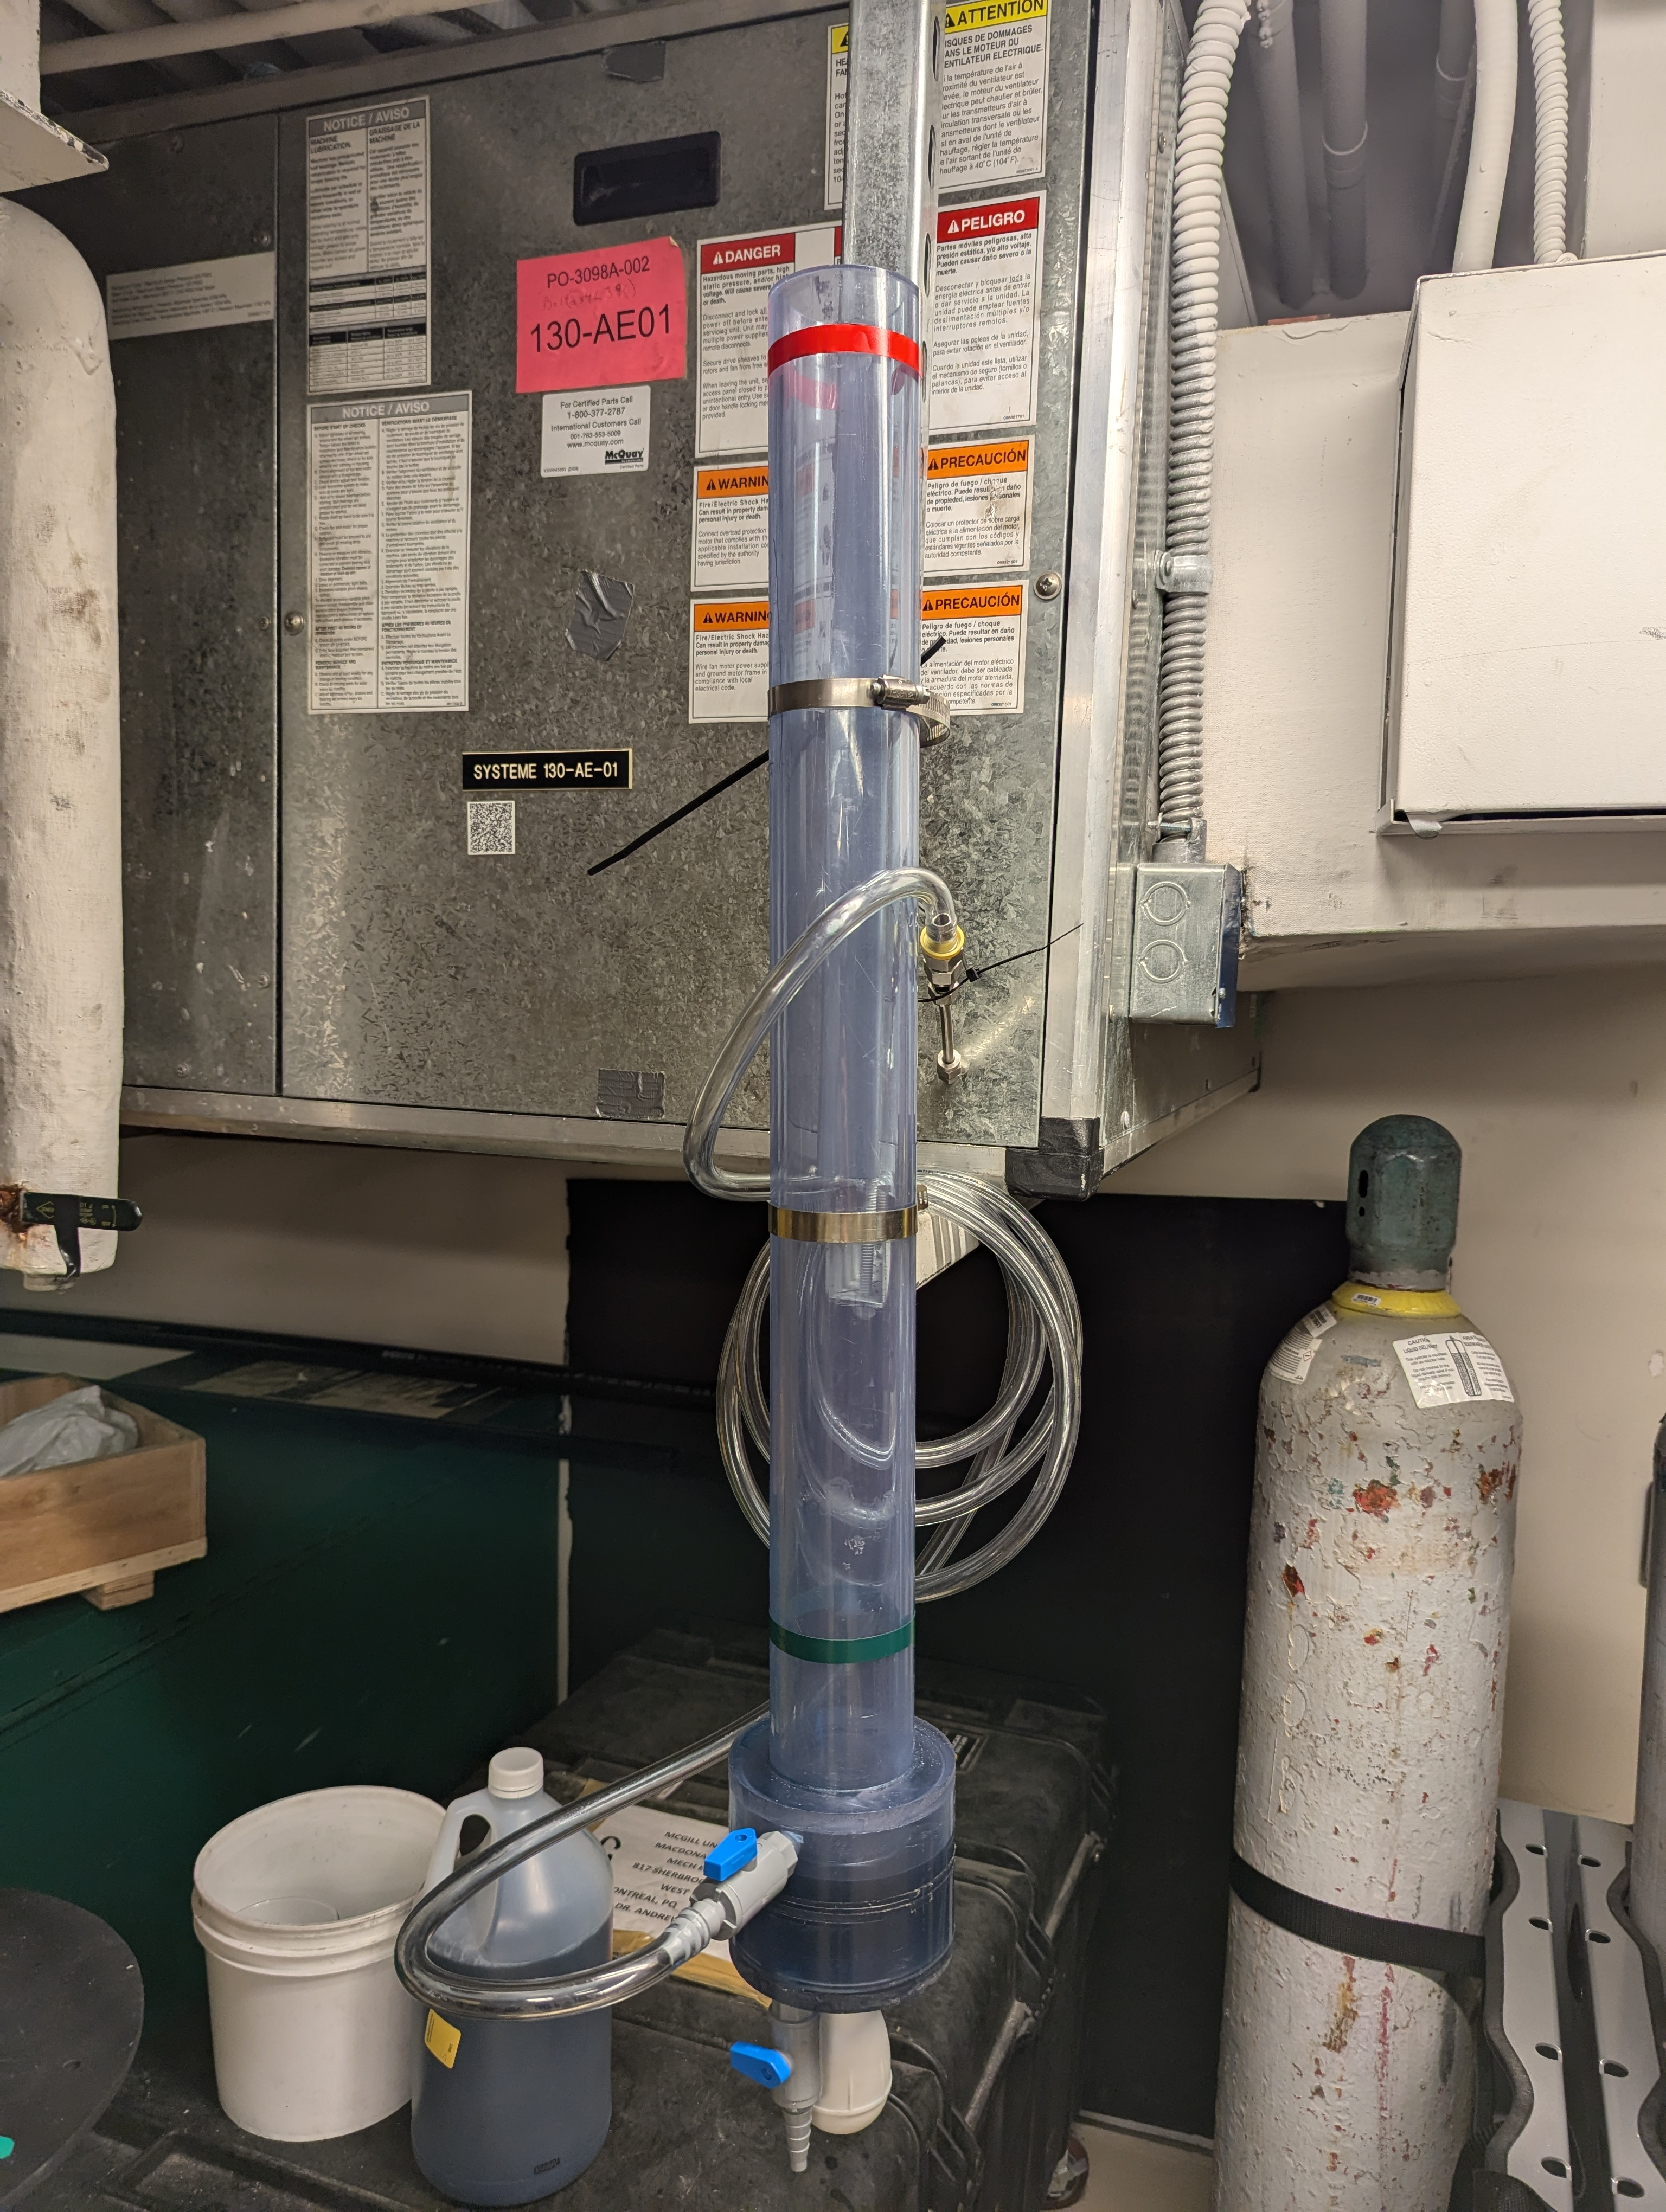
\includegraphics[width=0.5\textwidth]{assets/4 experiments/Bubble meter.png}
                \caption{Bubble meter setup}
                \label{fig:bubble meter}
            \end{figure}

            First, the valve was calibrated with air at \qtylist{3.45;6.89}{bar}. The valve was then calibrated with \qtylist{20;50}{bar} of argon. The volumetric flow rate was measured in both cases for increments of 0.50 rotations to 2.0 rotations. The calculated opening area of the valve is presented in \autoref{tab:opening_area}.

            \begin{table}[!ht]
                \centering
                \caption{Calculated Opening Area for Needle Valve at Different Rotations (Upstream Pressure = \qty{5000}{kPa} and Outlet Pressure = \qty{100}{kPa}), adapted from \autoref{chp:app Thariq}}
                \label{tab:opening_area}
                \begin{tabular}{|c|c|c|c|c|}
                \hline
                \textbf{Increment} & \textbf{Volume Flow (L/s)} & \textbf{Mass Flow (g/s)} & \textbf{Area (mm²)} & \textbf{Diameter (mm)} \\ \hline
                0.50 & 0.25 & 0.410 & 0.028 & 0.188 \\ \hline
                1.00 & 0.37 & 0.607 & 0.041 & 0.229 \\ \hline
                1.10 & 0.51 & 0.836 & 0.057 & 0.269 \\ \hline
                1.20 & 0.67 & 1.099 & 0.075 & 0.308 \\ \hline
                1.30 & 0.97 & 1.591 & 0.108 & 0.371 \\ \hline
                1.40 & 1.24 & 2.033 & 0.138 & 0.419 \\ \hline
                \end{tabular}
            \end{table}

            Assuming that the temperature inside V2 during CW LSP thrust tests is \qty{1200}{K} and the mass flow rate is \qty{0.641}{g/s}, \autoref{chp:app Thariq} recommends a rotation increment of approximately 1.33 to produce an $A^*$ of \qty{0.147}{mm^2}.

        \subsection{Summary of results}

            \autoref{tab:characteristics} presents a summary of the results determined from cold flow thruster characterization.

            \begin{table}[!ht]
                \centering
                \caption{Summary of the studied V2 thruster characteristics}
                \label{tab:characteristics}
                \begin{tabularx}{\textwidth}{XX}
                \toprule
                Characteristic                                          &     Value and unit          \\ \midrule
                Needle valve A* with predicted experiment conditions   &     \qty{0.147e-6}{m^2}     \\
                Nozzle A*                                               &     \qty{3.46e-8}{m^2}      \\
                Internal volume of thruster in flowing configuration    &     \qty{9.68e-6}{m^3}      \\
                Average cold flow thrust at 20 bar                      &     \qty{0.96}{N}           \\
                \bottomrule 
                \end{tabularx}
            \end{table}

        

    \section{Initial QCW LSP thrust tests (hot fire)}
 
        With V2 CW LSP achieved, and the cold flow thrust tests completed, initial QCW LSP thrust tests were attempted. The needle valve was not installed as it was not yet procured. 

        \begin{figure}[!ht]
            \centering
            \begin{subfigure}[t]{0.45\textwidth}
                \centering
                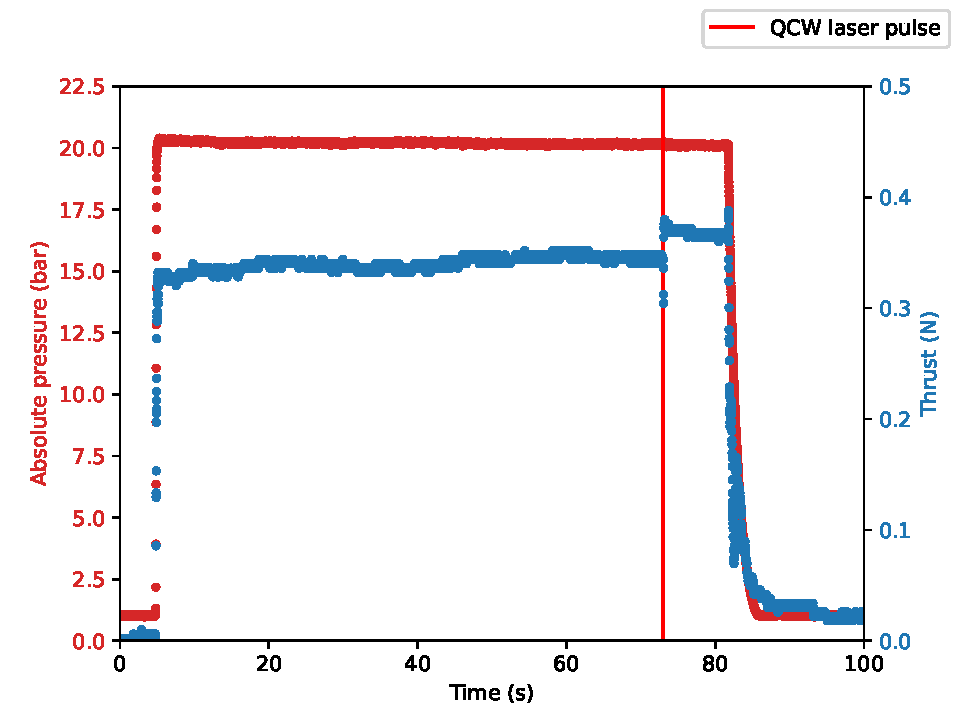
\includegraphics[width=\textwidth]{assets/4 experiments/LSP314.pdf}
                \caption{LSP314\_V2\_Flow3}
            \end{subfigure}
            \hfill
            \begin{subfigure}[t]{0.45\textwidth}
                \centering
                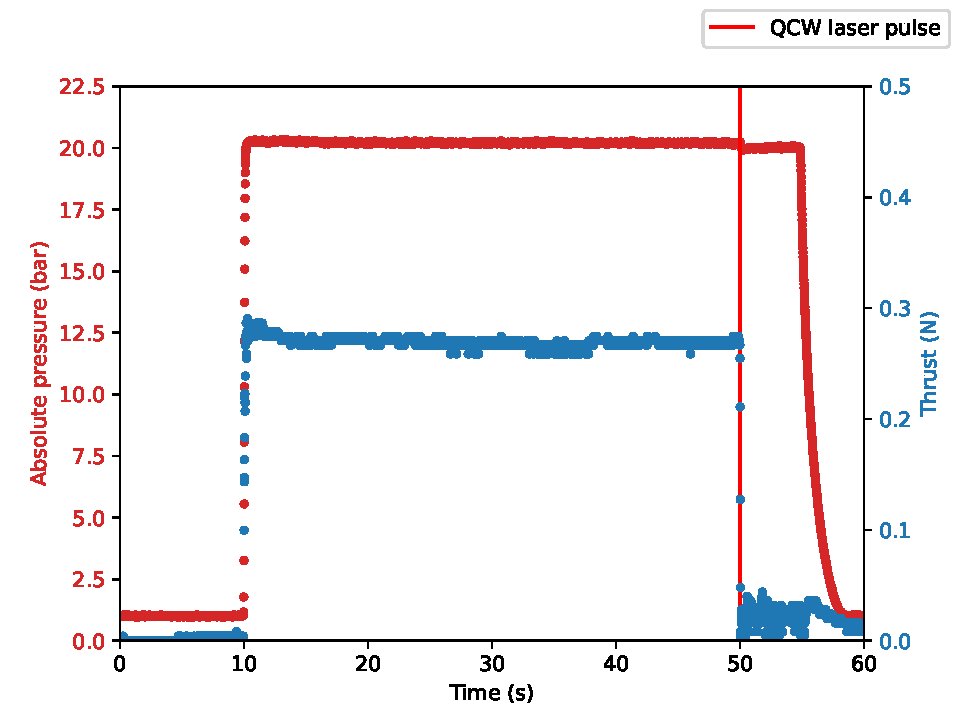
\includegraphics[width=\textwidth]{assets/4 experiments/LSP315.pdf}
                \caption{LSP315\_V2\_Flow4}
            \end{subfigure}
            \caption{Two QCW thrust tests}
            \label{fig:QCW LSP thrust tests}
        \end{figure}

        The thrust stand was unfortunately not calibrated before these tests. Thrust values should be closer to \qty{1}{N}, according to previous cold flow data. Nonetheless, the QCW pulse changes the thrust in both cases, but in opposing directions. No concrete increase in thrust could be determined with the current V2 setup when the laser was on.

        The following webcam frame (\autoref{fig:nozzle ablation}) was taken from the LSP315\_V2\_Flow4 \qty{3079}{W} QCW shot, with the electrodes unplugged so no LSP could be initiated. A plasma plume still left the nozzle and the noise of the flow changed once the laser was fired, indicating possible nozzle ablation.

        \begin{figure}[!ht]
            \centering
            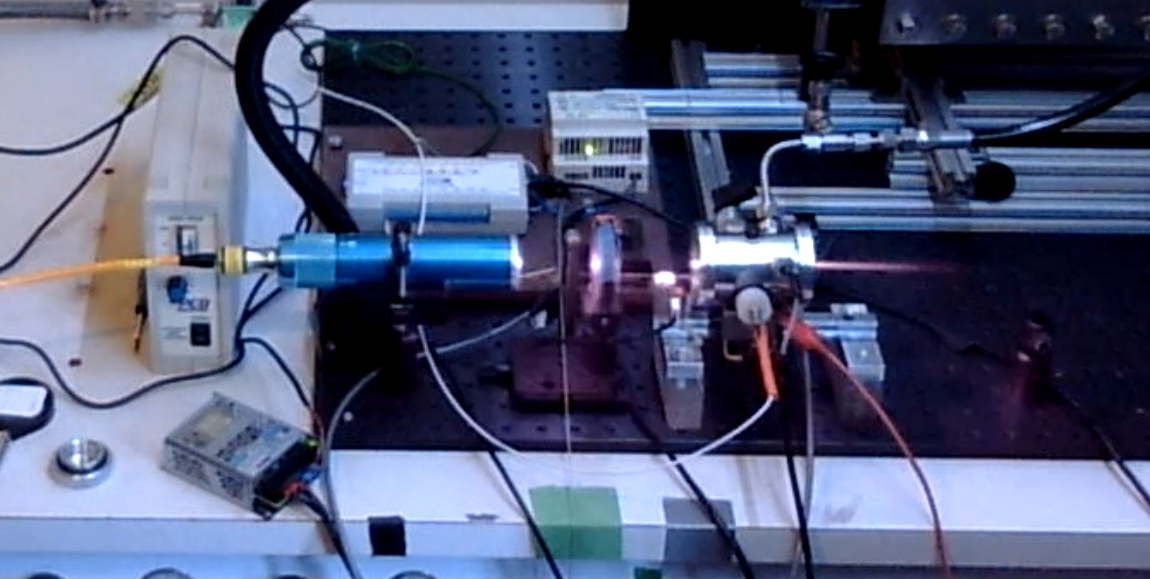
\includegraphics[width=0.5\textwidth]{assets/5 discussion/Nozzle ablation.png}
            \caption{Nozzle ablation during flowing test. LSP315\_V2\_Flow4.}
            \label{fig:nozzle ablation}
        \end{figure}

        Further flowing tests confirmed that LSP could be initiated by a spark in flowing argon. The following frame (\autoref{fig:V2 Flowing LSP}) from the Photron SA5 shows LSP light emission in \qty{20.0}{bar} of flowing argon.

        \begin{figure}[!ht]
            \centering
            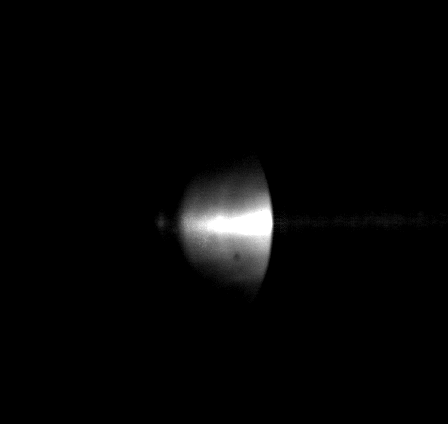
\includegraphics[width=0.45\textwidth]{assets/4 experiments/LSP321_V2_FLOW10.png}
            \caption{V2 Flowing QCW LSP. LSP321\_V2\_Flow10.}
            \label{fig:V2 Flowing LSP}
        \end{figure}

        



